\documentclass[12pt]{article}
\usepackage{setspace}
\onehalfspacing

\usepackage[UTF8]{ctex}

\usepackage{amsmath}
\usepackage{graphicx}
\usepackage[colorlinks=true, allcolors=blue]{hyperref}
\usepackage{tabularx}
\usepackage{booktabs}
\usepackage{textcomp}
\usepackage{makecell}
\usepackage{graphicx}
\usepackage{subcaption}
\usepackage{listings}
\usepackage{xcolor}
\usepackage{fontspec}
\usepackage{bm}
\usepackage{siunitx}
\usepackage{mathtools}
\usepackage{amssymb}

\usepackage[backend=biber, style=numeric, sorting=none]{biblatex}
\bibliography{references}

\title{逆问题数学模型与MR重建}
\author{甘嘉程}
\date{2026年7-8月}

\usepackage[a4paper,top=1.5cm,bottom=1.5cm,left=1.5cm,right=1.5cm]{geometry}
\linespread{1.5}
\begin{document}

\maketitle

\begin{abstract}
本报告基于《Magnetic Resonance Image Reconstruction: Theory, Methods, and Applications》第二章内容，从逆问题的数学描述出发，通过数学推导梳理了MR重建的完整理论框架。报告先说明了MR重建作为欠定逆问题的数学本质，随后处理k空间信号的离散化过程，之后在独立同分布Gaussian噪声假设下由最大似然估计推导最小二乘目标函数，得到Moore-Penrose广义逆形式的重建解。通过引入正则化方法，建立了欠定问题下唯一稳定解的求解框架。最后将线圈灵敏度、运动场、弛豫参数等未知量纳入编码矩阵，讨论了非线性逆问题求解策略。

本报告对文章原文的数学推导进行了进一步勘误与补全，在学习中，我针对原文省略的部分数学推导过程，结合自己的线性代数知识薄弱之处，进行了相关学习并以脚注形式补充了数学推导过程。在这个过程中，我进一步加深了对于成像算法数学原理的理解，受益匪浅。
\end{abstract}

\section{逆问题求解概述}
正问题（forward problem）指的是在已知输入（原因）的前提下，预测系统输出（效应）的过程。其逆过程即为逆问题（inverse problem）\footnote{逆问题：由测量结果（电磁感应信号）反推原因（磁化强度分布）的过程。其数学表达为：$\bm{s}=\mathbf{E}\bm{x}$，求$\bm{x}$。}。

逆问题可以通过其适定性分为两类。具体地，同时满足三个Hadamard条件\footnote{Hadamard条件（\autoref{fig:wellposed}）：1）解的存在性；2）解的唯一性；3）解的稳定性（即对采集数据的微小扰动应仅引起解的微小变化）。}的问题称为适定（well-posed）问题；若违反其中一个或多个条件，则称为不适定（ill-posed）问题。求解不适定逆问题时，通常需要对解施加额外约束，以找到合适的解。
\begin{figure}[h]
    \centering
    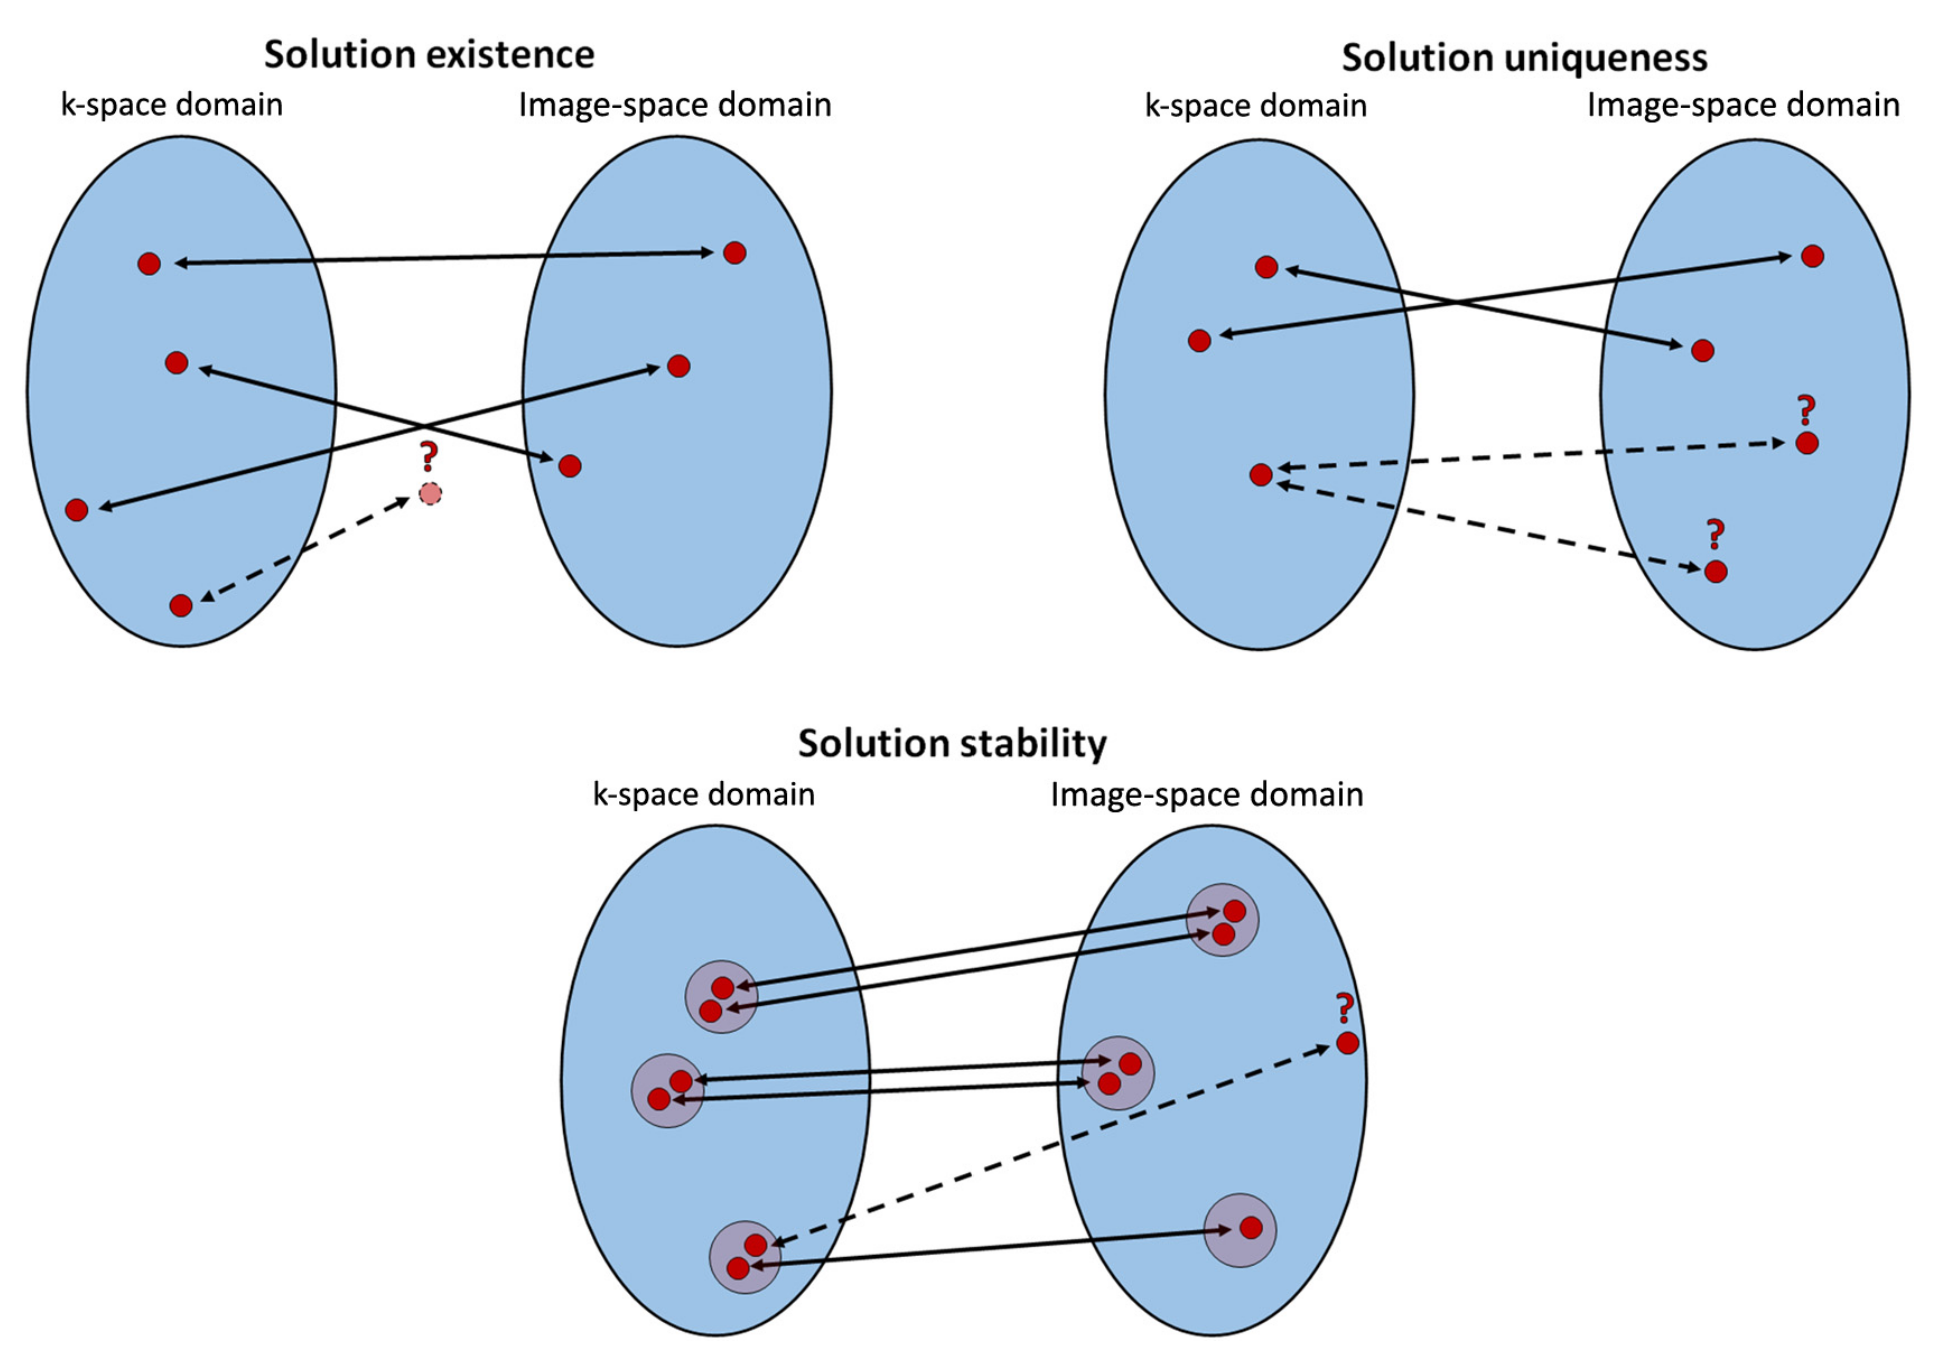
\includegraphics[width=\textwidth]{wellposed.png}
    \caption{三个Hadamard条件示意图}
    \label{fig:wellposed}
\end{figure}

MR重建通常是一个不适定的逆问题。针对三个Hadamard条件具体来说，如果没有正确采集感应信号$S(\bm{k})$，则解可能不存在（无解）。此外，我们希望从离散（有限）的采样中重建物体磁化强度的连续（无限）分布，该逆问题显然存在无穷多个解，不满足解的唯一性。特别地，将这类问题称为欠定（underdetermined）问题\footnote{欠定（Underdetermined）与欠采样（Undersampling）：由于未知量数（像素个数）大于有效方程数（k空间采样点数），造成的解不唯一的不适定问题。不同类型的欠采样如\autoref{fig:under}所示}。稳定性条件涉及采样的扰动对解的影响程度。由于
\begin{equation}
    \lim_{k\to\infty}\mathcal{F}\{\sin(kx\pi)\}=0
\end{equation}
一个高频扰动$\sin(kx\pi)$，尽管只会导致采样$\Delta S(\bm{k})$的微小变化，但在图像空间可能引起$\delta M(\bm{r})$的任意大变化。换言之，对高频扰动的敏感性导致了Fourier变换的不稳定性，通常表现为噪声放大。
\begin{figure}[h]
    \centering
    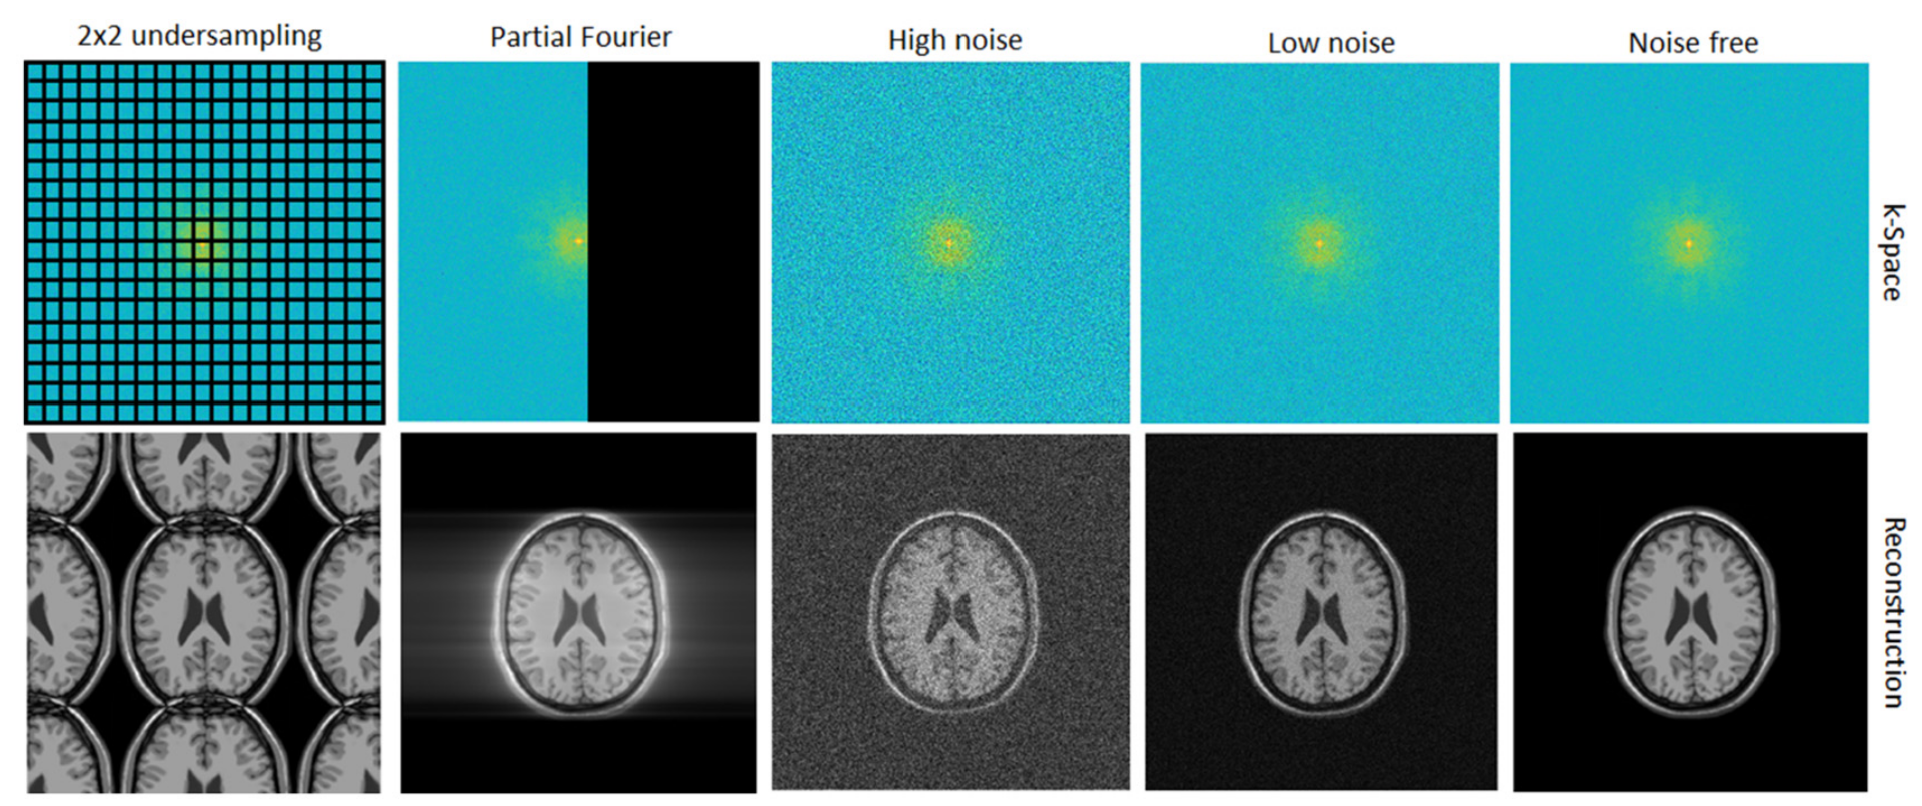
\includegraphics[width=\textwidth]{under.png}
    \caption{不同类型欠采样、噪声示意图}
    \label{fig:under}
\end{figure}

综上所述，MR信号重建，本质上是一个不适定（通常欠定）逆问题的求解过程。在信号采集阶段，通过施加梯度场和射频脉冲，在接收线圈中感应出时变电压，即k空间信号$S(\bm{k})$。经过空间离散化后，正问题可建模为线性方程组
\begin{equation}
    \bm{s}=\mathbf{E}\bm{x}
\end{equation}
其中$\bm{x}$代表待重建的磁化强度图像（像素向量），$\mathbf{E}$为编码矩阵（含Fourier变换、线圈灵敏度等），$\bm{s}$为离散化信号（k-空间向量）。

在实际测量中，数字信号采样还包含噪声，在独立同分布Gaussian噪声假设下，最合理的估计是使预测值与真实值的误差平方和最小，即最小二乘问题
\begin{equation}
    \hat{\bm{x}}=\arg\min_{\bm{x}}\|\bm{s}-\mathbf{E}\bm{x}\|_2^2
\end{equation}

如前文所述，在实际情况下，该最小二乘问题通常是欠定的，导致解不唯一。为了挑选唯一且合理的解，须引入额外的先验信息，称为约束或正则化项，这一过程称为正则化\footnote{约束（Constraint）与正则化（Regularization）：从物理角度类比，在欠定反演中，数据保真项（最小二乘项）的解集构成一个“平坦谷底”，即出现多重简并解。正则化可以类比为额外施加一个势阱$R(x)$（即约束），迫使在“平坦谷底”上选出唯一稳定解，从而破除简并。从数学上理解，正则化将欠定问题改造为
\begin{equation}
    \hat{\bm{x}}=\arg\min_{\bm{x}}\{\mathcal{D}(\bm{s},\mathbf{E}\bm{x})+\lambda \mathcal{R}(\bm{x})\}
\end{equation}
式中$\mathcal{D}$为数据保真项（类比驱动力），$\mathcal{R}$为正则泛函（类比势场）。}。将正则化项$\mathcal{R}(\bm{x})$加入目标函数
\begin{equation}
    \hat{\bm{x}}=\arg\min_{\bm{x}}\{\|\bm{s}-\mathbf{E}\bm{x}\|_2^2+\lambda\mathcal{R}(\bm{x})\}
\end{equation}
其中$\lambda$称为正则化系数\footnote{正则化系数$\lambda$：类比拉格朗日乘子法，$\lambda$起到调控数据保真项（$\mathcal{D}$）与约束项（$\mathcal{R}$）之间的平衡，可在物理上类比于系统的“刚度因子”。当$\lambda\to0$时，系统刚度趋零，解完全由（叠加噪声的）观测数据决定，可能出现“鬼影”；$\lambda\to\infty$ 时，系统趋于刚性，解退化至先验信息，过度正则化使得细节丢失。}。

当先验信息本身也未知（如线圈灵敏度、运动情况、组织本征参数等），问题退化为非线性逆问题，此时需采用非线性方法联合估计图像和模型参数。接下来，我们将从连续MR信号的离散化开始，按上述逻辑阐述MR重建的一般方法。

\section{MR信号的离散化}
第一章阐述了测量信号$S(\bm{k})$与成像物体横向磁化强度$M_{xy}(\bm{r})$之间的关系（忽略弛豫效应和接收线圈灵敏度分布）\footnote{勘误：原文p39(2.1)为$S(\bm{k})=\mathcal{F}\{M_{xy}(\bm{r})\}$，实际上由于电磁感应信号应考虑磁化强度的质子密度加权累计，等号应该为正比号。原文可能为了便于数学推导写成等号，本文为了物理上严谨，将在后文（\autoref{equ:2.1}、\autoref{equ:2.4}等）中使用正比号}
\begin{equation}
    S(\bm{k})\propto\int_{V} M_{xy}(\bm{r})e^{-2\pi i\bm{k}\cdot\bm{r}} d\bm{r}=\mathcal{F}\{M_{xy}(\bm{r})\}
    \label{equ:2.1}
\end{equation}
其中$\mathcal{F}$为Fourier变换，$\bm{r}=(x,y,z)$为图像空间坐标；$\bm{k}=(k_x,k_y,k_z)$为k空间坐标，满足$\bm{k}=\int_{0}^{t}(\gamma/2\pi)\bm{G}(\tau) d\tau$。\autoref{equ:2.1}描述了MR信号采集的正演模型。

在实际采样中，需要对MR信号进行离散化，得到一个离散且在$\pm k_{max}$范围内的带限数字信号$S(\bm{k}_n)$
\begin{equation}
    S(\bm{k}_n)=S(\bm{k})\sum_{-k_{\max}}^{+k_{\max}}\delta(\bm{k}-n\Delta\bm{k})=\Pi\left(\frac{\bm{k}}{2\bm{k}_{\max}}\right)S(\bm{k})\sum_{-\infty}^{+\infty}\delta(\bm{k}-n\Delta\bm{k})
    \label{equ:2.2}
\end{equation}
其中$\Pi$为矩形函数\footnote{勘误：原文p39(2.3)(2.4)将$\Pi\left(\frac{\bm{k}}{2\bm{k}_{\max}}\right)$误写成$\Pi\left(\frac{\bm{k}}{\bm{k}_{\max}}\right)$。按照$\Pi$函数的定义
\begin{equation}
    \Pi(t)=
    \begin{cases}
        1, & |t|\leq1/2 \\
        0, & |t|>1/2
    \end{cases}
\end{equation}
要使$\bm{k}$的截断频率在$\pm\bm{k}_{max}$，则$\Pi$函数应写成$\Pi\left(\frac{\bm{k}}{2\bm{k}_{\max}}\right)$}
\begin{equation}
    \Pi\left(\frac{\bm{k}}{2\bm{k}_{max}}\right)=
    \begin{cases}
        1, & \bm{k}\leq\bm{k}_{max} \\
        0, & \bm{k}>\bm{k}_{max}
    \end{cases}
\end{equation}

对\autoref{equ:2.2}进行逆Fourier变换并应用卷积定理
\begin{equation}
    \begin{aligned}
        \mathcal{F}^{-1}\left\{S(\bm{k}_n)\right\}
        &=\mathcal{F}^{-1}\left\{\Pi\left(\frac{\bm{k}}{2\bm{k}_{\max}}\right)S(\bm{k})\sum_{-\infty}^{+\infty}\delta(\bm{k}-n\Delta\bm{k})\right\} \\
        &=\mathcal{F}^{-1}\left\{\Pi\left(\frac{\bm{k}}{2\bm{k}_{\max}}\right)\right\}*\mathcal{F}^{-1}\{S(\bm{k})\}*\mathcal{F}^{-1}\left\{\sum_{-\infty}^{+\infty}\delta(\bm{k}-n\Delta\bm{k})\right\} \\
        &\propto2\bm{k}_{\max}\operatorname{sinc}(\bm{r}2\pi\bm{k}_{\max})*M_{xy}(\bm{r})*\frac{1}{\Delta\bm{k}}\sum_{-\infty}^{+\infty}\delta\left(\bm{r}-\frac{n}{\Delta\bm{k}}\right) \\
        &=\operatorname{sinc}(\bm{r}2\pi\bm{k}_{\max})*\frac{2\bm{k}_{\max}}{\Delta\bm{k}}\sum_{-\infty}^{+\infty}M_{xy}\left(\bm{r}-\frac{n}{\Delta\bm{k}}\right)
    \end{aligned}
    \label{equ:2.4}
\end{equation}

\autoref{equ:2.4}正比于$\sum_{-\infty}^{+\infty}M_{xy}\left(\bm{r}-\frac{n}{\Delta\bm{k}}\right)$，表明离散采样产生无限多个与$M_{xy}(\bm{r})$相同的重建图像$M_{xy}\left(\bm{r}-\frac{n}{\Delta\bm{k}}\right)$，其间距为$1/\Delta\bm{k}$（\autoref{fig:fourier}）。因此，视场$\mathbf{FOV}=(x_{\max}, y_{\max}, z_{\max})$可以表述为
\begin{equation}
    \boxed{\mathbf{FOV}=\frac{1}{\Delta\bm{k}}},\quad i.e. \quad\mathrm{FOV}_i=\frac{1}{\Delta k_i}, i=x,y,z
    \label{equ:2.5}
\end{equation}
若成像物体在$\mathbf{FOV}$外，则会出现$M_{xy}(\bm{r})$与$M_{xy}(\bm{r}\pm n/\Delta\bm{k})$的混叠伪影。至此，我们可以对“欠采样”进行第二种定义：若$\Delta\bm{k}^{-1}<\mathbf{FOV}$，则重建为欠采样的；同理，若$\Delta\bm{k}^{-1}=\mathbf{FOV}$，则为全采样的；若$\Delta\bm{k}^{-1}>\mathbf{FOV}$，则为过采样的。
\begin{figure}[h]
    \centering
    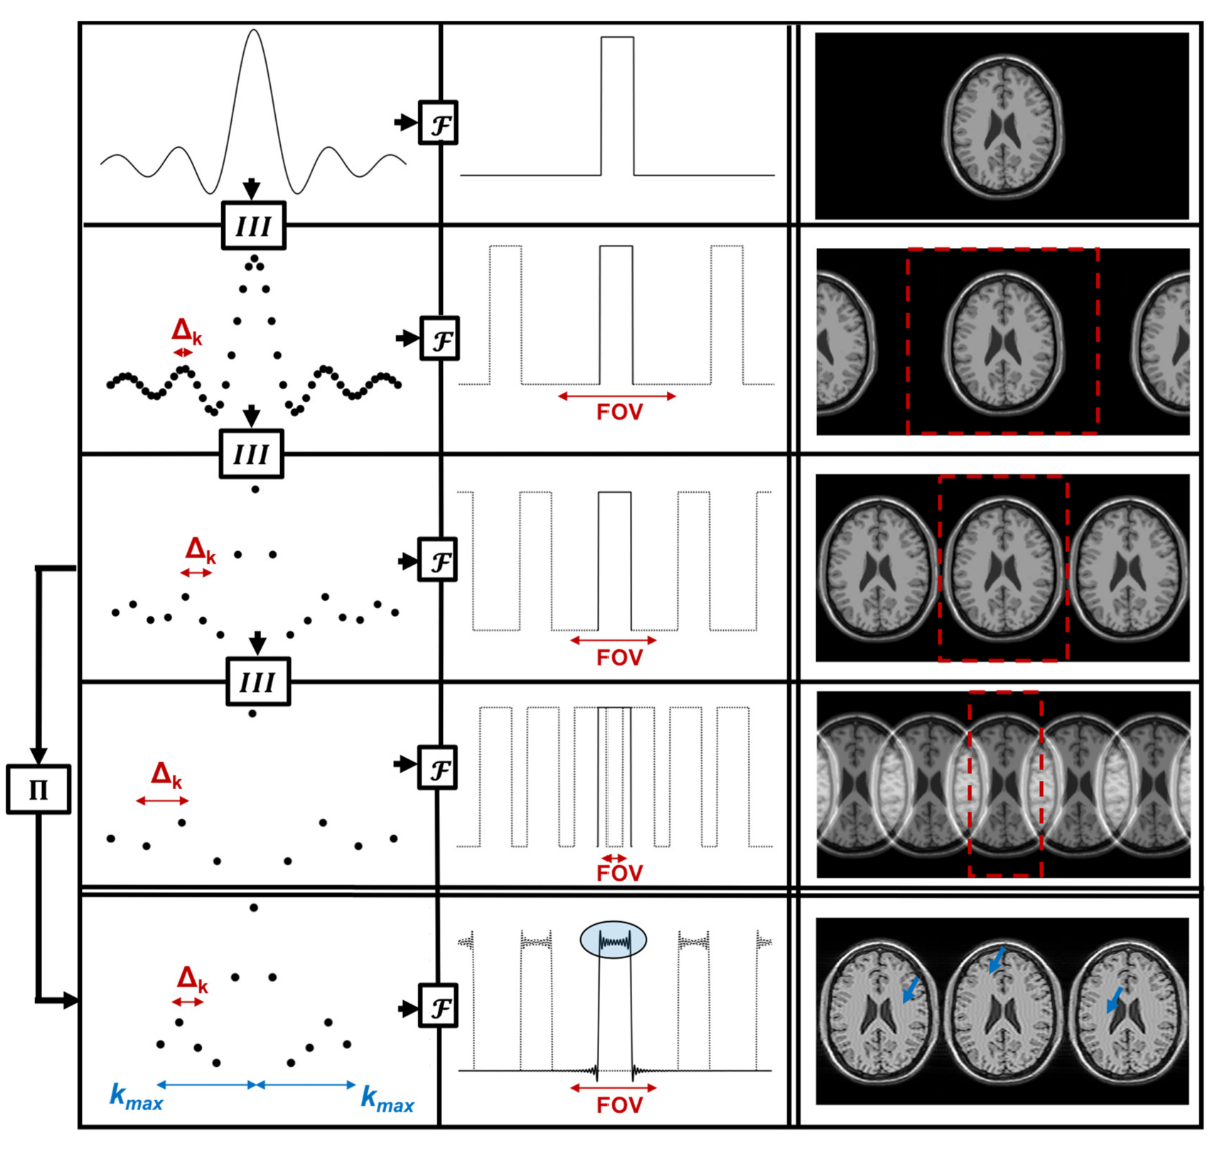
\includegraphics[width=\textwidth]{fourier.png}
    \caption{不同类型欠采样示意图}
    \label{fig:fourier}
\end{figure}

另一方面，\autoref{equ:2.4}的结果是原始信号$M_{xy}(\bm{r})$与$\operatorname{sinc}(\bm{r}2\pi k_{\max})$的卷积，这是由于采集的数字信号是带限的（\autoref{fig:fourier}）。卷积模糊原始信号，由此产生的空间分辨率
\begin{equation}
    \boxed{\Delta\bm{r}=\int_{-\infty}^{+\infty}\operatorname{sinc}(\bm{r}2\pi\bm{k}_{\max})d\bm{r}=\frac{1}{2\bm{k}_{\max}}}
    \label{equ:2.6}
\end{equation}

接下来我们将横向磁化矢量$M_{xy}(\bm{r})$进行空间离散化，使其可解\footnote{离散化与正则化的区别在于，其本质是把一个不可解的无限维问题变成可以计算的有限维欠定问题，而并没有解决欠定问题本身（不保证解的唯一性）。正则化则（在离散化的基础上）通过施加约束确保了解得存在唯一性。}
\begin{equation}
    M_{xy}(\bm{r})=\sum_{n=1}^{N_{\mathrm{pixels}}} M_{xy}(\bm{r}_n)b(\bm{r}-\bm{r}_n)
    \label{equ:2.8}
\end{equation}
其中$b(\bm{r}-\bm{r}_n)$为离散化基函数，人为选定矩形函数$b(\bm{r})=\Pi\left(\bm{r}/\Delta\bm{r}\right)$将横向磁化强度离散化为像素。

若物体全采样（即成像物体在$\mathbf{FOV}$范围内），则\autoref{equ:2.4}中$\sum_{-\infty}^{+\infty}M_{xy}\left(\bm{r}-\frac{n}{\Delta\bm{k}}\right)$仅保留$M_{xy}(\bm{r})$一项。结合\autoref{equ:2.4}、\autoref{equ:2.5}、\autoref{equ:2.6}和\autoref{equ:2.8}可得
\begin{equation}
    \begin{aligned}
        \mathcal{F}^{-1}\{S(\bm{k}_n)\}
        &\propto\operatorname{sinc}\left(\frac{\bm{r}\pi}{\Delta\bm{r}}\right)*\frac{2\bm{k}_{\max}}{\mathbf{FOV}}\sum_{n=1}^{N_{\mathrm{pixels}}} M_{xy}(\bm{r}_n)\Pi\left(\frac{\bm{r}-\bm{r}_n}{\Delta\bm{r}}\right) \\
        &=\boxed{\operatorname{sinc}\left(\frac{\bm{r}\pi}{\Delta\bm{r}}\right)*N_\mathrm{pixels}\sum_{n=1}^{N_{\mathrm{pixels}}} M_{xy}(\bm{r}_n)\Pi\left(\frac{\bm{r}-\bm{r}_n}{\Delta\bm{r}}\right)} \\
    \end{aligned}
    \label{equ:2.9}
\end{equation}
至此我们发现，k-空间的离散采样直接进行Fourier逆变换，会在图像域施加三个物理约束——视场由采样间距决定（\autoref{equ:2.5}）、空间分辨率由最大采样频率决定（\autoref{equ:2.6}）、以及由带限截断导致的sinc卷积模糊（Gibbs ringing）。经\autoref{equ:2.8}的空间离散化后，连续正演模型（\autoref{equ:2.4}）转化为有限个像素的求和（\autoref{equ:2.9}），保证了逆问题的可解性。需要指出的是，\autoref{equ:2.9}模型的适用范围是：无噪声、全采样、单通道Fourier编码。

\section{线性逆问题建模}
在本节中，我们回到\autoref{equ:2.1}\footnote{从本节开始，为了便于线性方程组书写，并且从物理实际中逐步抽象出线性数学模型，我们将\autoref{equ:2.1}的正比号改写成等号，并在后文中沿用这一写法。}，将连续的横向磁化强度$M_{xy}(\bm{r})$按\autoref{equ:2.8}进行离散化，展开为Fourier级数
\begin{equation}
    S(\bm{k}_n)=\mathcal{F}\{M_{xy}(\bm{r}_n)\}=\sum_{n=1}^{N_{\mathrm{pixels}}} M_{xy}(\bm{r}_n)b(\bm{r}-\bm{r}_n)e^{-2\pi i\bm{k}_n\cdot\bm{r}_n}\Delta\bm{r}\propto\Delta\bm{r}
    \label{equ:2.10}
\end{equation}
将该离散正演模型抽象为线性模型\footnote{假设像素足够小，使得体素内的磁化强度变化可以忽略，并用体素中心近似。}\footnote{同第一章，本文也通过不同字体区分矩阵和向量。具体来说，用加粗正体（如$\mathbf{E}$）来表示矩阵（二阶张量）；用加粗斜体（如$\bm{x}$）来表示向量（一阶张量）。}
\begin{equation}
    \boxed{\bm{s}=\mathbf{E}\bm{x}}
    \label{equ:2.11}
\end{equation}
其中$\bm{s}=(s_1,s_2,\cdots,s_m)^T$是k-空间数据向量（$m$维复向量；$m$即为采样数），$\bm{x}=(x_1,x_2,\cdots,x_n)^T$是图像空间向量（$n$维实向量；且$m<n$时为欠采样，$m=n$时为全采样），$\mathbf{E}$（一个$m\times n$复矩阵）是描述采集过程的编码矩阵，包含Fourier变换及离散化基$b$、弛豫或接收线圈阵列的空间灵敏度等其他纳入正演模型的运算。

引入离散线性模型（\autoref{equ:2.11}）具有三方面优势：（1）编码矩阵$\mathbf{E}$不局限于Fourier矩阵，而是可包含线圈灵敏度、场不均匀性、非笛卡尔轨迹等因素；（2）可引入加性噪声模型（\autoref{equ:2.12}），并通过MLE导出最小二乘目标函数（\autoref{equ:2.18}），这是线性重建的统计学基础；（3）可利用线性代数一般方法求解逆问题（无需\autoref{equ:2.9}的卷积计算）。

\autoref{equ:2.9}揭示了离散k-空间采样在图像域施加的若干物理约束，其为\autoref{equ:2.10}的构建提供了物理边界条件（\autoref{equ:2.5}、\autoref{equ:2.6}）。若脱离\autoref{equ:2.9}约束的离散化参数（$\Delta\bm{r}$、$\mathbf{FOV}$）和Gibbs ringing产生条件（sinc卷积），\autoref{equ:2.10}将退化为一个失去物理约束的纯数学离散化。

假设噪声为加性白Gaussian噪声$\bm{\varepsilon}$，则
\begin{equation}
    \bm{s}=\mathbf{E}\bm{x}+\bm{\varepsilon}
    \label{equ:2.12}
\end{equation}
为了在Gaussian噪声$\bm{\varepsilon}$存在的情况下估计$\bm{x}$，我们使用最大似然估计（Maximum Likelihood Estimation），求图像估计$\hat{\bm{x}}$，使得在给定图像$\bm{x}$条件下测到k-空间数据$\bm{s}$的条件概率最大化，即
\begin{equation}
    \hat{\bm{x}}=\arg\max_{\bm{x}} p(\bm{s}|\bm{x})
    \label{equ:2.13}
\end{equation}

假设噪声为独立同分布（i.i.d.）Gaussian分布
\begin{equation}
    \bm{\varepsilon}\sim\mathcal{N}\left(z;\mu,\sigma^2\right)=\frac{1}{\sqrt{2\pi\sigma^2}} e^{-\frac{(z-\mu)^2}{2\sigma^2}}
    \label{equ:2.14}
\end{equation}
其中$\mu=0$为均值，$\sigma$为标准差。因此\autoref{equ:2.13}中的条件概率为\footnote{证明：对于第$i$个采样点，噪声
\begin{equation}
    \varepsilon_i=s_i-(\mathbf{E}\bm{x})_i
    \label{equ:fn1}
\end{equation}
服从一维零均值Gaussian分布$\mathcal{N}(0,\sigma^2)$，概率密度函数为
\begin{equation}
    p(\varepsilon_i)=\frac{1}{\sqrt{2\pi\sigma^2}}e^{-\frac{\varepsilon_i^2}{2\sigma^2}}
    \label{equ:fn2}
\end{equation}

由于$\varepsilon_i$是$s_i$在给定$\bm{x}$下的误差，将\autoref{equ:fn1}代入\autoref{equ:fn2}可得观测到$s_i$的条件概率
\begin{equation}
    p(s_i|\bm{x})=\frac{1}{\sqrt{2\pi\sigma^2}}e^{-\frac{\left[s_i-(\mathbf{E}\bm{x})_i\right]^2}{2\sigma^2}}
\end{equation}
基于i.i.d.Gaussian分布假设，各点联合条件概率为
\begin{equation}
    p(\bm{s}|\bm{x})=\prod_{i=1}^{m} p(s_i|\bm{x})
\end{equation}
}
\begin{equation}
    p(\bm{s}|\bm{x})=\prod_{i=1}^{m}\frac{1}{\sqrt{2\pi\sigma^2}} e^{-\frac{\left[s_i-(\mathbf{E}\bm{x})_i\right]^2}{2\sigma^2}}
    \label{equ:2.15}
\end{equation}
其中$m$为采样数。因此\footnote{注意到log是单调递增函数，则$\arg\max_{\bm{x}}f(\bm{x})=\arg\max_{\bm{x}}\log f(\bm{x})$}
\begin{equation}
    \begin{aligned}
        \hat{\bm{x}}=\arg\max_{\bm{x}}\log p(\bm{s}|\bm{x})
        &=\arg\max_{\bm{x}}\left\{m\log\frac{1}{\sqrt{2\pi\sigma^2}}-\sum_{i=1}^{m}\frac{\left[s_i-(\mathbf{E}\bm{x})_i\right]^2}{2\sigma^2}\right\} \\
        &=\arg\min_{\bm{x}}\sum_{i=1}^{m} \left[s_i-(\mathbf{E}\bm{x})_i\right]^2
        \label{equ:2.16}
    \end{aligned}
\end{equation}
我们发现，上式即为最小二乘代价函数，将其写为$\ell_2$范数\footnote{$\ell_2$范数：对向量$\bm{x}=(x_1,x_2,\ldots,x_n)^T$，其$\ell_2$范数
\begin{equation}
    \|\bm{x}\|_2\equiv\sqrt{\sum_{i=1}^{n}|x_i|^2}
\end{equation}
即欧氏空间中各分量平方和的平方根，几何上表示向量的欧氏长度。最小化$\ell_2$范数等价于最小二乘准则，倾向于将误差均匀分布在各分量上，得到的解较为平滑但通常不稀疏。

与之相对，$\ell_1$范数
\begin{equation}
    \|\bm{x}\|_1\equiv\sum_{i=1}^{n}|x_i|
\end{equation}
即各分量绝对值之和，几何上表示Manhattan距离。最小化$\ell_1$范数会使解中许多分量为零，从而得到稀疏解。}形式
\begin{equation}
    \boxed{\hat{\bm{x}}=\arg\min_{\bm{x}}\|\bm{s}-\mathbf{E}\bm{x}\|_2^2}
    \label{equ:2.18}
\end{equation}
需要指出，本节推导的最小二乘形式\autoref{equ:2.18}基于i.i.d.Gaussian噪声假设，若使用不同噪声模型将导致不同的形式。

\section{线性逆问题的求解}\label{chap:2.4}
为便于后文讨论，我们设\footnote{勘误：原文p44(2.22)-(2.24)存在多处指标错误、共轭未写出的问题。本文进行了更规范的约定：1）对于复数$a$，其复共轭记为$a^*$；2）对于复矩阵$\mathbf{E}$，其第$i$行第$j$列分量记为$E_{ij}(i=1,\cdots,m;j=1,\cdots,n)$；3）使用Einstein求和约定：若$\mathbf{C}=\mathbf{A}\mathbf{B}$，则$\mathbf{C}$的各分量记为$C_{ik}=A_{ij} B_{jk}$，重复哑指标求和。在\autoref{equ:2.23}中将详细展示正确的计算过程。}
\begin{equation}
    \begin{aligned}
        f(\bm{x})=\|\bm{s}-\mathbf{E}\bm{x}\|_2^2
        &=(\bm{s}-\mathbf{E}\bm{x})^H(\bm{s}-\mathbf{E}\bm{x}) \\
        &=\left(s_j^*-x_i E_{ji}^*\right)\left(s_j-E_{ji} x_i\right)
        \label{equ:2.19}
    \end{aligned}
\end{equation}
其中$H$为Hermitian转置\footnote{Hermitian转置：$\mathbf{A}^H\equiv\left(\mathbf{A}^T\right)^*$，且对于复向量$\bm{a}$有
\begin{equation}
    \|\bm{a}\|_2^2=\bm{a}^H\bm{a}=\sum |a_i|^2
\end{equation}
即$\bm{a}^H\bm{a}$的值为复向量$\bm{a}$的模长平方。}。由此可得$f(\bm{x})$关于$\bm{x}$第$n$个分量的偏导数\footnote{注意到$E^i_j$不依赖于$x_n$（视为常数）；且$\frac{\partial x_i}{\partial x_n}=\delta_{in}$。}
\begin{equation}
    \begin{aligned}
        \widetilde{\frac{\partial f}{\partial x_n}}&=\left(\frac{\partial s_j^*}{\partial x_n}-\frac{\partial}{\partial x_n}x_i E_{ji}^*\right)\left(s_j-E_{ji} x_i\right)+\left(s_j^*-x_i E_{ji}^*\right)\left(\frac{\partial s_j}{\partial x_n}-\frac{\partial}{\partial x_n}E_{ji} x_i\right) \\
        &=\left(0-\delta_{in}E_{ji}^*\right)\left(s_j-E_{ji} x_i\right)+\left(s_j^*-x_i E_{ji}^*\right)\left(0 - E_{ji}\delta_{in}\right) \\
        &=-E_{jn}^* s_j+E_{jn}^* E_{ji} x_i-s_j^* E_{jn}+x_i E_{ji}^* E_{jn}
    \end{aligned}
    \label{equ:2.23}
\end{equation}
我们发现上式计算出的偏导数是一个复数，而回顾\autoref{equ:2.19}对$f(\bm{x})$的最小二乘定义，注意到其是$\bm{x}$的实函数，且$\bm{x}$为实向量，因此其梯度也应为实向量。由此，实际偏导数应取\autoref{equ:2.23}的实部\footnote{对任意复数$z$，$z+z^*=2\mathrm{Re}(z)$。对于\autoref{equ:2.23}中的四项，注意到：
\begin{enumerate}
    \item 第1、3项：令$z=E_{jn}^* s_j$，其复共轭为$z^*=(E_{jn}^* s_j)^*=E_{jn} s_j^*$，于是
    \begin{equation}
        -E_{jn}^* s_j-s_j^* E_{jn}=-2\mathrm{Re}\bigg[E_{jn}^* s_j\bigg]
    \end{equation}
    \item 第2、4项：类似地，令$w=E_{jn}^* E_{ji} x_i$，则
    \begin{equation}
        E_{jn}^* E_{ji} x_i+x_i E_{ji}^* E_{jn}=2\mathrm{Re}\bigg[E_{jn}^* E_{ji} x_i\bigg]
    \end{equation}
\end{enumerate}
}，即
\begin{equation}
    \begin{aligned}
        \frac{\partial f}{\partial x_n}
        &=-2\mathrm{Re}\bigg[E_{jn}^*\left(s_j-E_{ji} x_i\right)\bigg]
        =-2\mathrm{Re}\bigg[E_{jn}^*\left[s_j-(\mathbf{E}\bm{x})_j\right]\bigg] \\
        &=-2\mathrm{Re}\bigg[\left(\mathbf{E}^H\right)_{nj}\left[s_j-(\mathbf{E}\bm{x})_j\right]\bigg]
        =-2\mathrm{Re}\bigg[\left[\mathbf{E}^H\left(\bm{s}-\mathbf{E}\bm{x}\right)\right]_n\bigg]
    \end{aligned}
    \label{equ:2.24}
\end{equation}

将上式结果推广到梯度算符
\begin{equation}
    \nabla f=\left[\frac{\partial f}{\partial x_1},\cdots,\frac{\partial f}{\partial x_N}\right]^T=-2\mathrm{Re}\bigg[\mathbf{E}^H(\bm{s}-\mathbf{E}\bm{x})\bigg]
    \label{equ:2.25}
\end{equation}
若在$\hat{\bm{x}}$的局部$f$满足一阶条件$\nabla f(\hat{\bm{x}})=\bm{0}$，则$\hat{\bm{x}}$是$f$的最小值点\footnote{$f$为最小二乘函数，在数学上是凸函数，因此一阶导数零点恰为极小值点、稳定点。}。由此得到
\begin{align}
    \mathrm{Re}\bigg[\mathbf{E}^H(\bm{s}-\mathbf{E}\hat{\bm{x}})\bigg]&=\bm{0} \\
    \Aboxed{\mathrm{Re}\bigg[\mathbf{E}^H\mathbf{E}\bigg]\hat{\bm{x}}&=\mathrm{Re}\bigg[\mathbf{E}^H\bm{s}\bigg]}
    \label{equ:2.25a}
\end{align}
本节上述推导及正规方程\footnote{正规方程（Normal Equation）：在最小二乘问题$\min_{\bm{x}}\|\mathbf{A}\bm{x}-\bm{b}\|_2^2$中，令目标函数梯度为零所得的线性方程组，形如
\begin{equation}
    \mathbf{A}^H\mathbf{A}\bm{x}=\mathbf{A}^H\bm{b}
\end{equation}
其系数矩阵$\mathbf{A}^H\mathbf{A}$具有对称/共轭对称性。}\autoref{equ:2.25a}对任意矩阵$\mathbf{E}$均成立。当全采样或过采样（$m\ge n$）时，$\mathbf{E}$通常是列满秩矩阵，此时$\mathrm{Re}[\mathbf{E}^H\mathbf{E}]$可逆；当欠采样（$m<n$）时$\mathrm{Re}[\mathbf{E}^H\mathbf{E}]$不可逆，要求解$\hat{\bm{x}}$需引入正则化条件（见\autoref{chap:2.5}）。本节后文推导适用于第一种情形，可由正规方程\autoref{equ:2.25a}直接解出最一般的显式解\footnote{\autoref{equ:2.25b}中$\mathrm{Re}[\cdot]$分别作用于矩阵和向量之后再求逆相乘，不可将$\mathrm{Re}[\cdot]$提取到括号外部。}
\begin{equation}
    \hat{\bm{x}}=\mathrm{Re}\bigg[\mathbf{E}^H\mathbf{E}\bigg]^{-1}\mathrm{Re}\bigg[\mathbf{E}^H\bm{s}\bigg]
    \label{equ:2.25b}
\end{equation}

在全采样（及过采样）笛卡尔采样下，编码矩阵可以简化为
\begin{equation}
    \mathbf{E}=\mathbf{F}\mathbf{C}
\end{equation}
其中$\mathbf{F}$为Fourier编码矩阵，$\mathbf{C}$为线圈灵敏度矩阵（对于单通道采集，$\mathbf{C}=\mathbf{I}$；对于多通道并形成像，$\mathbf{C}\neq\mathbf{I}$），并且$\mathbf{F}$是一个酉矩阵即$\mathbf{F}^H\mathbf{F}=\mathbf{I}$\footnote{证明：设归一化DFT矩阵$\mathbf{F}$的元素为
\begin{equation}
    F_{kn}=\frac{1}{\sqrt{N}}e^{-i2\pi\frac{kn}{N}}\quad k,n=1,2,\cdots,N
\end{equation}
考察
\begin{equation}
    (\mathbf{F}^H\mathbf{F})_{mn}=\sum_{k=1}^{N} \frac{1}{\sqrt{N}}e^{i2\pi\frac{km}{N}}\cdot\frac{1}{\sqrt{N}}e^{-i2\pi\frac{kn}{N}}=\frac{1}{N}\sum_{k=1}^{N} e^{i2\pi\frac{k(m-n)}{N}}=
    \begin{cases} 1&\quad m=n \\ 0&\quad m\neq n \end{cases}
    \text{（正交归一性）}
\end{equation}
因此$(\mathbf{F}^H\mathbf{F})_{mn}=\delta_{mn}$，即$\mathbf{F}^H\mathbf{F}=\mathbf{I}$。}。代入式(\autoref{equ:2.25b})得
\begin{equation}
    \begin{aligned}
        \hat{\bm{x}}
        &=\mathrm{Re}\bigg[(\mathbf{F}\mathbf{C})^H(\mathbf{F}\mathbf{C})\bigg]^{-1}\mathrm{Re}\bigg[(\mathbf{F}\mathbf{C})^H\bm{s}\bigg] \\
        &=\mathrm{Re}\bigg[\mathbf{C}^H\mathbf{F}^H\mathbf{F}\mathbf{C}\bigg]^{-1}\mathrm{Re}\bigg[\mathbf{C}^H\mathbf{F}^H\bm{s}\bigg] \\
        &=\mathrm{Re}\bigg[\mathbf{C}^H\mathbf{C}\bigg]^{-1}\mathrm{Re}\bigg[\mathbf{C}^H\mathbf{F}^{-1}\bm{s}\bigg]
        \label{equ:2.26}
    \end{aligned}
\end{equation}

特别地，若线圈灵敏度可近似为实矩阵，则$\mathbf{C}^H\mathbf{C}=\mathbf{C}^T\mathbf{C}$为实对称矩阵，故$\mathrm{Re}[\mathbf{C}^H\mathbf{C}]=\mathbf{C}^H\mathbf{C}$。由于待重建的横向磁化强度$M_{xy}(\bm{r})$为实物理量，其Fourier变换具有Hermitian对称性，因此$\mathbf{F}^{-1}\bm{s}$为实向量\footnote{证明：Hermitian对称性的数学描述
\begin{equation}
    S(\bm{k})=S^*(-\bm{k})
\end{equation}
对k-空间数据$s(\bm{k})$，其逆Fourier变换及复共轭
\begin{align}
    M(\bm{r})&=\mathcal{F}\{s(\bm{k})\}=\int s(\bm{k})e^{i2\pi\bm{k}\cdot\bm{r}}d\bm{k} \\
    M^*(\bm{r})&=\int s^*(\bm{k})e^{-i2\pi\bm{k}\cdot\bm{r}}d\bm{k}=\int s^*(-\bm{k}')e^{i2\pi\bm{k}'\cdot\bm{r}}d\bm{k}'
\end{align}
由Hermitian对称性
\begin{equation}
    M^*(\bm{r})=\int s(\bm{k}')e^{i2\pi\bm{k}'\cdot\bm{r}}d\bm{k}'=M(\bm{r})
\end{equation}
故$M(\bm{r})$为实函数。离散情形下对$\mathbf{F}^{-1}\bm{s}$同理：正频和负频分量互为复共轭，积分时虚部恰好抵消。}，且经实矩阵$\mathbf{C}^H=\mathbf{C}^T$加权后，$\mathbf{C}^H\mathbf{F}^{-1}\bm{s}$仍为实向量，故$\mathrm{Re}[\mathbf{C}^H\mathbf{F}^{-1}\bm{s}]=\mathbf{C}^H\mathbf{F}^{-1}\bm{s}$。在上述条件下，\autoref{equ:2.26}中两个取实部运算均可去掉
\begin{equation}
    \boxed{\hat{\bm{x}}=\left(\mathbf{C}^H\mathbf{C}\right)^{-1}\mathbf{C}^H\mathbf{F}^{-1}\bm{s}=\left(\mathbf{E}^H\mathbf{E}\right)^{-1}\mathbf{E}^H\bm{s}=\mathbf{E}^\dagger\bm{s}}
    \label{equ:2.27}
\end{equation}
其中$\mathbf{E}^\dagger$为Moore-Penrose广义逆\footnote{Moore-Penrose广义逆：对任意矩阵$\mathbf{A}$，其Moore-Penrose广义逆$\mathbf{A}^\dagger$是唯一满足以下四个Penrose条件的矩阵：
\begin{enumerate}
    \item $\mathbf{A}\mathbf{A}^\dagger\mathbf{A}=\mathbf{A}$
    \item $\mathbf{A}^\dagger\mathbf{A}\mathbf{A}^\dagger=\mathbf{A}^\dagger$
    \item $\mathbf{A}\mathbf{A}^\dagger$的厄米性：$(\mathbf{A}\mathbf{A}^\dagger)^H=\mathbf{A}\mathbf{A}^\dagger$
    \item $\mathbf{A}^\dagger\mathbf{A}$的厄米性：$(\mathbf{A}^\dagger\mathbf{A})^H=\mathbf{A}^\dagger\mathbf{A}$
\end{enumerate}
当$\mathbf{E}$列满秩且$\mathbf{C}$为实矩阵时，$\mathbf{E}^H\mathbf{E}$可逆，$\mathbf{E}^\dagger=(\mathbf{E}^H\mathbf{E})^{-1}\mathbf{E}^H$。更一般地，对于任意矩阵$\mathbf{E}$，其Moore-Penrose广义逆$\hat{\bm{x}}=\mathbf{E}^\dagger\bm{s}$恒为线性系统$\mathbf{E}\bm{x}=\bm{s}$的极小范数最小二乘解：列满秩时给出唯一最小二乘解，欠定时在无穷多最小二乘解中取范数最小者。}。需要强调的是，只有同时满足：1）$\mathbf{E}$是列满秩矩阵（全采样或过采样）；2）线圈灵敏度矩阵为实矩阵，正规方程\autoref{equ:2.25a}才可得到\autoref{equ:2.27}形式的解。

\section{欠定问题的求解：正则化}\label{chap:2.5}
接下来我们将讨论正规方程\autoref{equ:2.25a}在编码矩阵$\mathbf{E}$不满秩情况下的求解。回到\autoref{equ:2.18}，为在欠采样条件下获得唯一、稳定的解$\hat{\bm{x}}$，需要将额外的假设或先验信息纳入一个代价函数$\mathcal{R}(\bm{x})$，并将\autoref{equ:2.18}转化为正则化问题\footnote{正则化问题与约束问题等价，\autoref{equ:2.30}也可写成约束问题形式，即
\begin{equation}
    \begin{aligned}
        \hat{\bm{x}}&=\arg\min_{\bm{x}}\mathcal{R}(\bm{x}) \\
        &\text{满足约束} \|\bm{s}-\mathbf{E}\bm{x}\|_2^2<\bm{\varepsilon}
    \end{aligned}
    \label{equ:2.29}
\end{equation}
上式的含义是：在所有可能解中，选择在给定假设或先验信息下具有最小$\mathcal{R}(\bm{x})$的解，同时满足数据一致性的约束（即保持采样数据与待重建图像之间的一致）。
}
\begin{equation}
    \boxed{\hat{\bm{x}}=\arg\min_{\bm{x}}\{\|\bm{s}-\mathbf{E}\bm{x}\|_2^2+\lambda\mathcal{R}(\bm{x})\}}
    \label{equ:2.30}
\end{equation}
其中第一项为数据一致性\footnote{数据一致性（Data Consistency）：要求重建的图像数据$\bm{x}$必须能通过正演计算匹配采样数据$\bm{s}$，构成正则化问题中的约束。在数学上表述为$\|\bm{s}-\mathbf{E}\bm{x}\|_2^2<\bm{\varepsilon}$}约束，第二项为代价函数$\mathcal{R}(\bm{x})$的正则化参数$\lambda$加权项，该参数控制数据一致性与优化准则之间的权衡。如\autoref{fig:regularize}所示，将低分辨率先验图像作为正则化条件纳入含噪、欠采样图像，希望得到尽可能接近真实的重建图像。如果$\lambda$过小（欠正则化），此时约束项占主导，导致重建图像与无正则化时相似，呈现混叠和噪声放大；如果$\lambda$过大（过正则化），此时正则化项占主导，重建图像过度被“拉向”先验而导致分辨率损失。总的来说，$\lambda$会正向促进先验信息对解的影响，可能同时抑制噪声和与噪声水平相当的图像特征。适当选择$\lambda$可以在不损害对真实图像忠实度的前提下实现混叠和噪声的抑制。接下来讨论两种常见的正则化方式。
\begin{figure}[h]
    \centering
    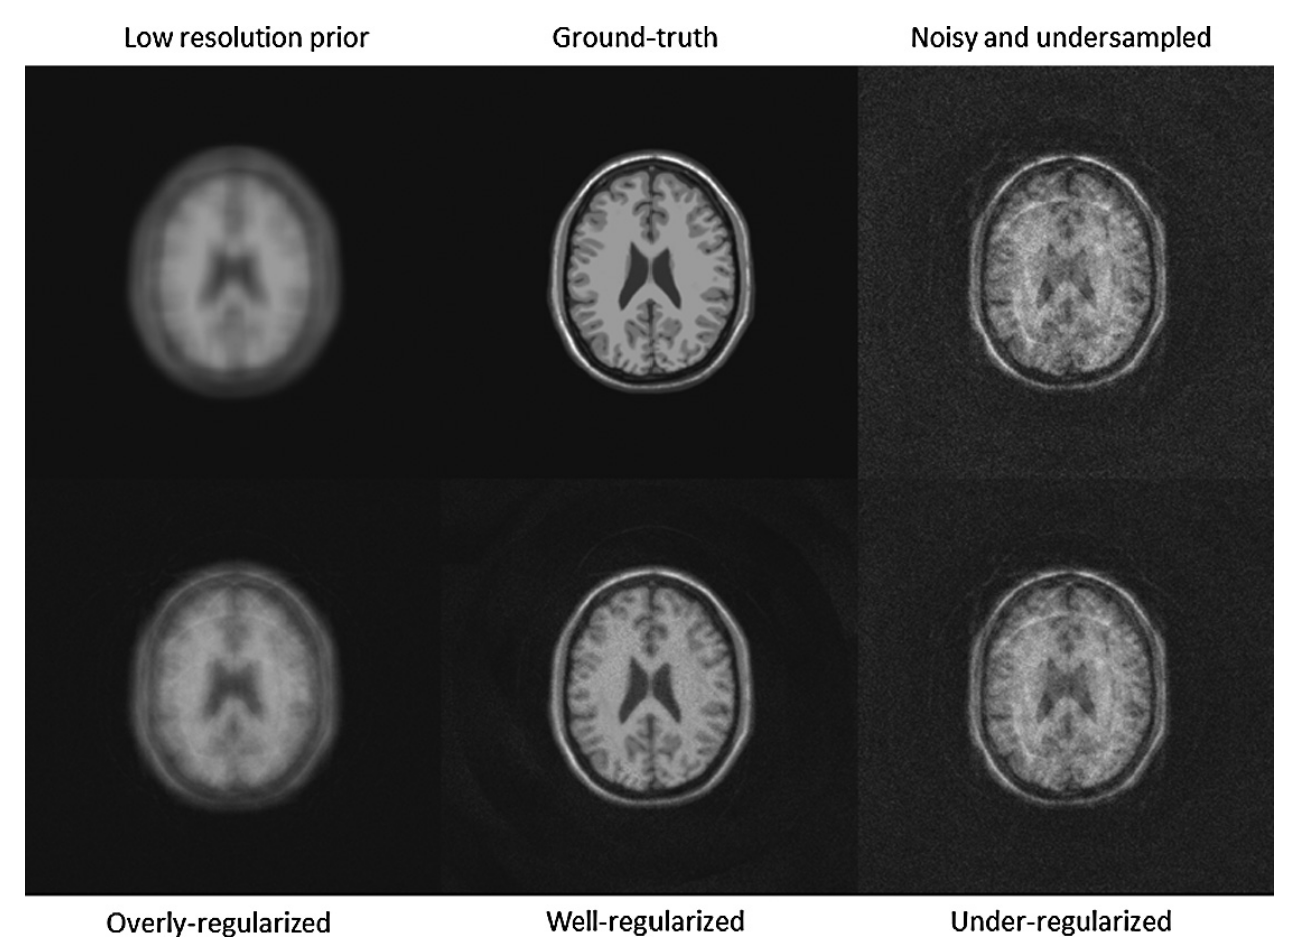
\includegraphics[width=0.8\textwidth]{regularize.png}
    \caption{不同程度正则化示意图}
    \label{fig:regularize}
\end{figure}

\subsection{$\ell_2$范数正则化（Tikhonov正则化）}
设图像$\bm{x}$的先验信息$\bm{x}^0=(x^0_1,x^0_2,\cdots,x^0_n)^T$，对应的$\ell_2$范数正则化问题
\begin{equation}
    \hat{\bm{x}}=\arg\min_{\bm{x}}f(\bm{x})=\arg\min_{\bm{x}}\{\|\bm{s}-\mathbf{E}\bm{x}\|_2^2+\lambda\|\bm{x}-\bm{x}^0\|_2^2\}
    \label{equ:2.32}
\end{equation}
其中代价函数$\mathcal{R}(\bm{x})=\|\bm{x}-\bm{x}^0\|_2^2$\footnote{$\ell_2$范数代价函数可类比谐振子势能（$V(x)=\frac{1}{2}k x^2$），其处处连续可微且恢复力$F=-\partial V_x=-kx$具有线性形式。因此，$\ell_2$范数正则化类似在向k-空间中心“拖拽”所有采样数据，如同在k-空间表面覆盖了一层弹性膜。$\ell_2$范数正则化将导致图像高频成分被平滑化。}，表示要求重建图像与先验信息在最小二乘意义下相似，称为Tikhonov正则化。类比\autoref{chap:2.4}中的分析，设
\begin{equation}
    f(\bm{x})=\|\bm{s}-\mathbf{E}\bm{x}\|_2^2+\lambda\|\bm{x}-\bm{x}^0\|_2^2=g(\bm{x})+\lambda h(\bm{x})
\end{equation}
分别计算偏导数得\footnote{证明：$\frac{\partial g}{\partial x_n}$的计算与\autoref{equ:2.19}-\autoref{equ:2.24}完全相同；由于$h(\bm{x})$是实函数且$\bm{x}$、$\bm{x}^0$均为实向量，导数必然为实
\begin{align}
    h(\bm{x})&=(\bm{x}-\bm{x}^0)^H(\bm{x}-\bm{x}^0)=(x_i-x^0_i)^2 \\
    \frac{\partial h}{\partial x_n}&=2\left(\frac{\partial x_i}{\partial x_n}-0\right)(x_i-x^0_i)=2\delta_{in}(x_i-x^0_i)=2I_{nj}I_{ji}(x_i-x^0_i)=2\left[\mathbf{I}^H\mathbf{I}(\bm{x}-\bm{x}^0)\right]_n
\end{align}
}
\begin{align}
    \frac{\partial g}{\partial x_n}&=-2\mathrm{Re}\bigg[\left[\mathbf{E}^H\left(\bm{s}-\mathbf{E}\bm{x}\right)\right]_n\bigg] \\
    \frac{\partial h}{\partial x_n}&=2\left[\mathbf{I}^H\mathbf{I}(\bm{x}-\bm{x}^0)\right]_n \\
    \frac{\partial f}{\partial x_n}&=\frac{\partial g}{\partial x_n}+\lambda\frac{\partial h}{\partial x_n} \\
    \nabla f&=-2\mathrm{Re}\bigg[\mathbf{E}^H\left(\bm{s}-\mathbf{E}\bm{x}\right)\bigg]+2\lambda\mathbf{I}^H\mathbf{I}(\bm{x}-\bm{x}^0)
    \label{equ:2.33}
\end{align}

加入一阶条件$\nabla f(\hat{\bm{x}})=\bm{0}$，可得正规方程
\begin{align}
    \mathrm{Re}\bigg[\mathbf{E}^H\left(\bm{s}-\mathbf{E}\bm{x}\right)\bigg]-\lambda\mathbf{I}^H\mathbf{I}(\bm{x}-\bm{x}^0)&=\bm{0} \\
    \left(\mathrm{Re}\bigg[\mathbf{E}^H\mathbf{E}\bigg]+\lambda\mathbf{I}\right)\hat{\bm{x}}&=\mathrm{Re}\bigg[\mathbf{E}^H\bm{s}\bigg]+\lambda\bm{x}^0
\end{align}
其中$\mathbf{I}$为单位矩阵，有$\mathbf{I}^H\mathbf{I}=\mathbf{I}$和$\mathbf{I}\bm{x}^0=\bm{x}^0$。与无正则化情形（\autoref{equ:2.25b}适用于列满秩矩阵$\mathbf{E}$）不同，上式的系数矩阵$\mathrm{Re}[\mathbf{E}^H\mathbf{E}]+\lambda\mathbf{I}$恒为正定矩阵\footnote{正定矩阵（Positive Definite Matrix）：对实对称矩阵$\mathbf{A}$，若对任意非零实向量$\bm{x}$均有$\bm{x}^T\mathbf{A}\bm{x}>0$，则称$\mathbf{A}$为正定矩阵。正定矩阵必可逆，否则存在$\bm{x}\neq\bm{0}$使$\mathbf{A}\bm{x}=\bm{0}$，导致$\bm{v}^T\mathbf{A}\bm{v}=0$，与定义矛盾。}\footnote{证明：首先，对任意实向量$\bm{x}$，考察二次型
\begin{equation}
    \bm{x}^T\mathrm{Re}\bigg[\mathbf{E}^H\mathbf{E}\bigg]\bm{x}=\mathrm{Re}\bigg[\bm{x}^T(\mathbf{E}^H\mathbf{E})\bm{x}\bigg]=\mathrm{Re}\bigg[(\mathbf{E}\bm{x})^H(\mathbf{E}\bm{x})\bigg]=\|\mathbf{E}\bm{x}\|_2^2\ge 0
\end{equation}
因此，对$\lambda>0$及任意$\bm{x}\neq\bm{0}$
\begin{equation}
    \bm{x}^T\left(\mathrm{Re}\bigg[\mathbf{E}^H\mathbf{E}\bigg]+\lambda\mathbf{I}\right)\bm{x}=\|\mathbf{E}\bm{x}\|_2^2+\lambda\|\bm{x}\|_2^2>0
\end{equation}
满足正定矩阵定义。由此可见，Tikhonov正则化能处理欠定问题的本质在于，$\lambda\mathbf{I}$项的加入保证了系数矩阵的可逆性。}，故对任意$\mathbf{E}$，系数矩阵始终可逆。因此，可以写出Tikhonov正则化问题的显式解
\begin{equation}
    \boxed{\hat{\bm{x}}=\left(\mathrm{Re}\bigg[\mathbf{E}^H\mathbf{E}\bigg]+\lambda\mathbf{I}\right)^{-1}\left(\mathrm{Re}\bigg[\mathbf{E}^H\bm{s}\bigg]+\lambda\bm{x}^0\right)}
    \label{equ:2.34}
\end{equation}

事实上，任意线性矩阵$\mathbf{L}$都可以包含在Tikhonov正则化项中，即
\begin{equation}
    \hat{\bm{x}}=\arg\min_{\bm{x}}\{\|\bm{s}-\mathbf{E}\bm{x}\|_2^2+\lambda\|\mathbf{L}\bm{x}-\bm{x}^0\|_2^2\}
\end{equation}
对应的解为
\begin{equation}
    \hat{\bm{x}}=\left(\mathrm{Re}\bigg[\mathbf{E}^H\mathbf{E}\bigg]+\lambda\mathrm{Re}\bigg[\mathbf{L}^H\mathbf{L}\bigg]\right)^{-1}\left(\mathrm{Re}\bigg[\mathbf{E}^H\bm{s}\bigg]+\lambda\mathrm{Re}\bigg[\mathbf{L}^H\bigg]\bm{x}^0\right)
    \label{equ:2.35}
\end{equation}

\subsection{$\ell_1$范数正则化}
压缩感知技术（第八章）采用$\ell_1$范数正则化。最小化某个向量$\bm{x}$的$\ell_1$范数的等价先验信息是：为$\bm{x}$施加稀疏约束。$\ell_1$正则化问题写为\footnote{$\ell_1$范数代价函数可类比于线性楔形势能$V(x)=k|x|$，其在零点处不可导，且广义恢复力在零点附近为常数。因此，$\ell_1$范数正则化倾向于将小幅震荡分量“锁定”在零态。$\ell_1$范数正则化图像的边缘结构几乎不变，而在平坦区域强制归零。}
\begin{equation}
    \hat{\bm{x}}=\arg\min_{\bm{x}}f(\bm{x})=\arg\min_{\bm{x}}\{\|\bm{s}-\mathbf{E}\bm{x}\|_2^2+\lambda\|\bm{\Phi}\bm{x}\|_1\}
    \label{equ:2.36}
\end{equation}
其中$\bm{\Phi}$为稀疏变换\footnote{稀疏变换（Sparsifying Transform）：若一个$p\times n$矩阵$\bm{\Phi}$，将$n$维（非稀疏）图像$\bm{x}$线性映射为向量$\bm{\alpha}=\bm{\Phi}\bm{x}$，满足$\bm{\alpha}$中仅有$k\ll p$个分量非零，则称$\bm{x}$在$\bm{\Phi}$下是$k$-稀疏的。$\ell_1$范数$\|\bm{\Phi}\bm{x}\|_1=\sum_j|\Phi_{ji}x_i|$度量了变换系数的稀疏程度。}。设
\begin{equation}
    f(\bm{x})=\|\bm{s}-\mathbf{E}\bm{x}\|_2^2+\lambda\|\bm{\Phi}\bm{x}\|_1=g(\bm{x})+\lambda\varphi(\bm{x})
\end{equation}

接下来分析对$\varphi(\bm{x})$求偏导数的过程。先来讨论，由于$y(x)=|x|$在$x=0$邻域内不可导，故采用光滑近似$y(x)\approx\sqrt{x^2+\epsilon}\ (\epsilon\ll 1)$使其在全定义域内可导，导函数为
\begin{equation}
    \frac{dy}{dx}\approx\frac{d}{dx}\sqrt{x^2+\epsilon}=\frac{x}{\sqrt{x^2+\epsilon}}
\end{equation}
由此计算$\varphi(\bm{x})=\|\bm{\Phi}\bm{x}\|_1=\sum_j|\Phi_{ji}x_i|$的偏导数\footnote{注意到对实变量$x$有$|x|=\sqrt{x^2}$，而$\bm{\Phi}$在压缩感知中通常为实矩阵，故$\Phi_{ji}x_i$恒为实数，$\varphi(\bm{x})$恒为实函数。}。
\begin{equation}
    \begin{aligned}
        \frac{\partial \varphi(\bm{x})}{\partial x_n}
        &=\frac{\partial}{\partial x_n}\sum_j|\Phi_{ji}x_i|
        =\frac{\partial}{\partial x_n}\sum_j\sqrt{(\Phi_{ji}x_i)^2+\epsilon} \\
        &=\sum_j\frac{\Phi_{ji}x_i}{\sqrt{(\Phi_{ji}x_i)^2+\epsilon}}\cdot\frac{\partial}{\partial x_n}(\Phi_{ji}x_i)
        =\sum_j\frac{\Phi_{ji}x_i}{\sqrt{(\Phi_{ji}x_i)^2+\epsilon}}\cdot\Phi_{ji}\delta_{in} \\
        &=\sum_j\frac{\Phi_{jn}\Phi_{ji}x_i}{\sqrt{(\Phi_{ji}x_i)^2+\epsilon}}
        =\sum_j\left(\bm{\Phi}^H\right)_{nj}W_{jj}\left(\bm{\Phi}\bm{x}\right)_j \\
        &=\left[\bm{\Phi}^H\mathbf{W}(\bm{x})\bm{\Phi}\bm{x}\right]_n
    \end{aligned}
    \label{equ:2.37}
\end{equation}
其中$\mathbf{W}(\bm{x})$为非独立于$\bm{x}$的对角加权矩阵，其对角元
\begin{equation}
    W_{jj}=\frac{1}{\sqrt{(\Phi_{ji}x_i)^2+\epsilon}}=\frac{1}{|(\bm{\Phi}\bm{x})_j|}
\end{equation}

由此可得稀疏正则化重建的梯度\footnote{勘误：原文p50(2.38)在稀疏变换项多了一个系数2，实际上该系数是对$\ell_2$范数平方项求导产生的，由$\ell_1$范数定义的正则化项并不会出现该系数。}
\begin{align}
    \frac{\partial f}{\partial x_n}&=\frac{\partial g}{\partial x_n}+\lambda\frac{\partial\varphi}{\partial x_n} \\
    \nabla f&=-2\mathrm{Re}\big[\mathbf{E}^H(\bm{s}-\mathbf{E}\bm{x})\big]+\lambda\bm{\Phi}^H\mathbf{W}(\bm{x})\bm{\Phi}\bm{x}
    \label{equ:2.38}
\end{align}
加入一阶条件$\nabla f(\hat{\bm{x}})=\bm{0}$可得
\begin{equation}
    \boxed{2\mathrm{Re}\big[\mathbf{E}^H(\bm{s}-\mathbf{E}\bm{x})\big]-\lambda\bm{\Phi}^H\mathbf{W}(\bm{x})\bm{\Phi}\bm{x}=\bm{0}}
    \label{equ:2.38a}
\end{equation}
由于$\mathbf{W}(\bm{x})$依赖于$\bm{x}$，正则化项是$\bm{x}$的非线性项。因此，由\autoref{equ:2.38a}无法得到关于$\bm{x}$的正规方程，也不能写出类似\autoref{equ:2.34}的显式解。$\ell_1$范数正则化问题的求解需要使用非线性方法（见第三章）。

\section{非线性逆问题}
当正向模型\autoref{equ:2.11}中的编码矩阵$\mathbf{E}$依赖需要估计的未知参数$\bm{\theta}$时，会产生非线性逆问题（通常是欠定的\footnote{即使数据是全采样的，非线性逆问题也可能由于高维度的参数空间而变为欠定问题，即$m<n+\theta_{\text{parameters}}$}，需正则化）
\begin{equation}
    \begin{aligned}
        \{\hat{\bm{x}},\hat{\bm{\theta}}\}&=\arg\min_{\bm{x},\bm{\theta}}g(\bm{x},\bm{\theta}) \\
        \Aboxed{&=\arg\min_{\bm{x},\bm{\theta}}\left\{\|\bm{s}-\mathbf{E}(\bm{\theta})\bm{x}\|_2^2+\lambda_x\mathcal{R}_x(\bm{x})+\lambda_\theta \mathcal{R}_\theta(\bm{\theta})\right\}}
    \end{aligned}
    \label{equ:2.39}
\end{equation}
接下来讨论非线性逆问题的三个典型例子：并行成像、运动校正和参数重建。

\subsection{非线性并行成像}
在并行成像中，设像素位置$r=1,2,\cdots,n$，采样通道编码$s=1,2,\cdots,l$。线圈灵敏度矩阵$\mathbf{C}=\operatorname{diag}(\mathbf{C}_1,\mathbf{C}_2,\ldots,\mathbf{C}_l)$是具有$l$个$n\times n$对角块的块对角复矩阵，其中第$s$个对角块是一个$n\times n$的对角方阵$\mathbf{C}_s=\operatorname{diag}(c_{1,s},c_{2,s},\cdots,c_{n,s})$，对角元$c_{r,s}$为待估计的非零元素。非线性并行成像将线圈灵敏度矩阵$\mathbf{C}$作为待估计参数纳入正演模型，即
\begin{equation}
    \mathbf{E}(\mathbf{C})=\mathbf{B}\mathbf{F}\mathbf{C}
\end{equation}
其中$\mathbf{B}$为k-空间采样矩阵（对角稀疏逻辑矩阵）。对于全采样数据（$m=n\times l$），必定有$m<n+n\times l$，因此非线性并行成像是一个欠定逆问题
\begin{equation}
    \{\hat{\bm{x}},\hat{\mathbf{C}}\}=\arg\min_{\bm{x},\mathbf{C}}\{\|\bm{s}-\mathbf{E}(\mathbf{C})\bm{x}\|_2^2+\sum_{i=\bm{x},\mathbf{C}} \lambda_i\mathcal{R}_i(\cdot)\}
    \label{equ:2.40}
\end{equation}
求解该问题有两种主要的非线性方法。

\subsubsection{Gauss-Newton方法}\label{chap:2.6.1.1}
在Gauss-Newton法中，将非线性逆问题描述为
\begin{equation}
    \widehat{\bm{E}}(\bm{y})=\bm{s}
    \label{equ:2.41.0}
\end{equation}
其中$\bm{y}=[x_1,\cdots,x_n,c_{1,1},\cdots,c_{n,l}]=[\bm{x},\mathbf{c}_1,\cdots,\mathbf{c}_l]$。$\widehat{\bm{E}}(\bm{y})$是一个从$n+n\times l$维到$m\times l$维的向量值函数（不再是矩阵），其第$s$个分量是一个$m$维列向量$\widehat{\bm{E}}_s$，可类比为一个独立工作的采样通道（其线圈灵敏度为$\mathbf{C}_s$），该通道的采样可描述为矩阵乘法形式
\begin{equation}
    \widehat{\bm{E}}_s=\mathbf{B}\mathbf{F}\mathbf{C}_s\bm{x}
\end{equation}
此外，$\bm{s}=(\bm{s}_1,\cdots,\bm{s}_l)^T$也不再是一个$m$维长列向量，而是一个具有$l$个$m$维分量的列向量（总长度$m\times l$）。因此
\begin{equation}
    \widehat{\bm{E}}(\bm{y})
    =\begin{pmatrix}
        \widehat{\bm{E}}_1(\bm{x},\mathbf{C}_1) \\
        \widehat{\bm{E}}_2(\bm{x},\mathbf{C}_2) \\
        \cdots \\
        \widehat{\bm{E}}_l(\bm{x},\mathbf{C}_l)
    \end{pmatrix}
    =\begin{pmatrix}
        \mathbf{B}\mathbf{F}\mathbf{C}_1\bm{x} \\
        \mathbf{B}\mathbf{F}\mathbf{C}_2\bm{x} \\
        \cdots \\
        \mathbf{B}\mathbf{F}\mathbf{C}_l\bm{x}
    \end{pmatrix}
    =\begin{pmatrix} \bm{s}_1 \\ \cdots \\ \bm{s}_l \end{pmatrix}
\end{equation}
因此可以计算$\widehat{\bm{E}}(\bm{y})$的偏导数
\begin{align}
    \frac{\partial\widehat{\bm{E}}_s(\bm{y})}{\partial\bm{x}}
    &=\frac{\partial}{\partial\bm{x}}\mathbf{B}\mathbf{F}\mathbf{C}_s\bm{x}=\mathbf{B}\mathbf{F}\mathbf{C}_s \\
    \frac{\partial\widehat{\bm{E}}_s(\bm{y})}{\partial\mathbf{C}_s}
    &=\frac{\partial}{\partial\mathbf{C}_s}\mathbf{B}\mathbf{F}\mathbf{C}_s\bm{x}=\frac{\partial}{\partial\mathbf{C}_s}[\mathbf{B}\mathbf{F}\cdot\operatorname{diag}(\bm{x})]\mathbf{C}_s=\mathbf{B}\mathbf{F}\cdot\operatorname{diag}(\bm{x})
\end{align}

Gauss-Newton方法的主要思路是在当前迭代解$\bm{y}^{[i]}$附近构建线性问题，并估计小量$d\bm{y}$。将正演模型（\autoref{equ:2.41.0}）Taylor展开到一阶\footnote{勘误：原文p51(2.41)对最后一个等号的处理缺乏严谨性，等式左边是对解的一阶近似，而右边是采样的精确值，二者并不相等。然而，本式说明了\autoref{equ:2.42}中最小二乘项的来历，该等号可以视作数据一致性的约束，故在本文中加以保留并作说明。}
\begin{equation}
    \widehat{\bm{E}}\left(\bm{y}^{[i]}+d\bm{y}\right)\approx\widehat{\bm{E}}\left(\bm{y}^{[i]}\right)+\mathcal{D}\widehat{\bm{E}}\left(\bm{y}^{[i]}\right)d\bm{y}=\bm{s}
    \label{equ:2.41}
\end{equation}
其中$\mathcal{D}$是Jacobian矩阵\footnote{Jacobian矩阵：对于一个向量值函数$\bm{F}(\bm{x}):\mathbb{R}^n\to\mathbb{R}^m$，其Jacobian矩阵$\mathbf{J}=\mathcal{D}\bm{F}$是一个$m\times n$矩阵，第$i$行第$j$列元素为$J_{ij}=\frac{\partial F_i}{\partial x_j}$。$\mathcal{D}\bm{F}$的每一行是$\bm{F}$各分量关于所有自变量的偏导数，几何上表示该函数在当前点的最佳线性逼近，即$d\bm{F}=\mathbf{J}\cdot d\bm{x}$}。为了从\autoref{equ:2.41}中求解合适的$d\bm{y}$，我们对$d\bm{y}$表述一个近似线性的正则化逆问题（用最小二乘估计）
\begin{equation}
    d\hat{\bm{y}}^{[i+1]}=\arg\min_{d\bm{y}}\left\{\left\|\bm{s}-\widehat{\bm{E}}\left(\bm{y}^{[i]}\right)-\mathcal{D}\widehat{\bm{E}}\left(\bm{y}^{[i]}\right)d\bm{y}\right\|_2^2+\lambda\mathcal{R}(d\bm{y})\right\}
    \label{equ:2.42}
\end{equation}
求解\autoref{equ:2.42}需要共轭梯度法（第三章），迭代求解$d\bm{y}$并更新$\bm{y}^{[i+1]}=\bm{y}^{[i]}+d\bm{y}^{[i]}$可得最终解$\hat{\bm{y}}$（形式还可能与初始条件$\bm{y}^{[0]}$有关）。

\subsubsection{参数化方法}\label{chap:2.6.1.2}
另一种处理非线性并行成像问题的方法是对线圈灵敏度进行参数化以减少未知数。由于线圈灵敏度足够光滑，可以用低阶多项式进行参数化
\begin{equation}
    c_{r,s}=\sum_{k=1}^{P} \alpha_{k,s}r^k
    \label{equ:2.43.0}
\end{equation}
其中$P$是多项式阶数，$P\ll n\times l$。因此，将对$\mathbf{C}$的估计从求解$c_{r,s}$转向求解系数$\alpha_{i,s}$可以显著减少未知数\footnote{勘误：原文p51-53(2.43)-(2.51)省略了正则化项，本文在后续章节中均加以补全，以延续逻辑一惯性。}由此我们可以得到非线性正则化逆问题
\begin{equation}
    \{\hat{\bm{x}},\hat{\bm{\theta}}\}=\arg\min_{\bm{x},\bm{\theta}}\left\{\|\bm{s}-\mathbf{B}\mathbf{F}\mathbf{C}(\bm{\theta})\bm{x}\|_2^2+\lambda_x\mathcal{R}_x(\bm{x})+\lambda_\theta\mathcal{R}_\theta(\bm{\theta})\right\}
    \label{equ:2.43}
\end{equation}
其中$\bm{\theta}=(\alpha_{1,1},\cdots,\alpha_{P,1};\cdots;\cdots,\alpha_{k,s},\cdots;\cdots;\alpha_{1,l},\cdots,\alpha_{P,l})^T$是包含全部$\alpha_{k,s}$的长列向量。使用交替最小化（第三章）进行迭代求解：固定一个变量而计算另一个变量，求解以下子问题
\begin{align}
    \hat{\bm{x}}^{[i+1]}&=\arg\min_{\bm{x}}\left\{\left\|\bm{s}-\mathbf{B}\mathbf{F}\mathbf{C}\left(\hat{\bm{\theta}}^{[i]}\right)\bm{x}\right\|_2^2+\lambda_x\mathcal{R}_x(\bm{x})\right\}
    \label{equ:2.44a} \\
    \hat{\bm{\theta}}^{[i+1]}&=\arg\min_{\bm{\theta}}\left\{\left\|\bm{s}-\mathbf{B}\mathbf{F}\mathbf{C}(\bm{\theta})\hat{\bm{x}}^{[i]}\right\|_2^2+\lambda_\theta\mathcal{R}_\theta(\bm{\theta})\right\}
    \label{equ:2.44b}
\end{align}
\autoref{equ:2.44a}是$\bm{x}$的线性逆问题；\autoref{equ:2.44b}包含了$\bm{\theta}$依赖的待估计参数$\mathbf{C}$，不是$\bm{\theta}$的线性逆问题，经过矩阵变换\footnote{证明：将线圈灵敏度矩阵$\mathbf{C}(\bm{\theta})$展开
\begin{equation}
    \mathbf{C}(\bm{\theta})=\begin{pmatrix}
        \mathbf{C}_1(\bm{\theta}) & & & \\
        & \mathbf{C}_2(\bm{\theta}) & & \\
        & & \ddots & \\
        & & & \mathbf{C}_l(\bm{\theta})
    \end{pmatrix}_{nl\times nl}=\begin{pmatrix}
        \operatorname{diag}(\bm{c}_1(\bm{\theta})) & & & \\
        & \operatorname{diag}(\bm{c}_2(\bm{\theta})) & & \\
        & & \ddots & \\
        & & & \operatorname{diag}(\bm{c}_l(\bm{\theta}))
    \end{pmatrix}
\end{equation}
其中$\bm{c}_s(\bm{\theta})=(c_{1,s}(\bm{\theta}),c_{2,s}(\bm{\theta}),\cdots,c_{n,s}(\bm{\theta}))$。在并形成像中，$\bm{x}$应为$n\times l$维列向量，即将$l$个$\bm{x}$纵向堆叠，这样计算$\mathbf{C}(\bm{\theta})\bm{x}$才能维度匹配得到一个$n\times l$维列向量。由此可以计算
\begin{equation}
    \mathbf{C}(\bm{\theta})\bm{x}=\begin{pmatrix}
        \mathbf{C}_1(\bm{\theta})\mathbf{x} \\
        \mathbf{C}_2(\bm{\theta})\mathbf{x} \\
        \vdots \\
        \mathbf{C}_l(\bm{\theta})\mathbf{x}
    \end{pmatrix}=\begin{pmatrix}
        (c_{1,1}(\bm{\theta})x_1,c_{2,1}(\bm{\theta})x_2,\cdots,c_{n,1}(\bm{\theta})x_n)^T \\
        (c_{1,2}(\bm{\theta})x_1,c_{2,2}(\bm{\theta})x_2,\cdots,c_{n,2}(\bm{\theta})x_n)^T \\
        \vdots \\
        (c_{1,l}(\bm{\theta})x_1,c_{2,l}(\bm{\theta})x_2,\cdots,c_{n,l}(\bm{\theta})x_n)^T
    \end{pmatrix}_{nl\times1}
\end{equation}
由多项式参数化\autoref{equ:2.43.0}可知
\begin{equation}
    c_{r,s}\cdot x_r=\left(\sum_{k=1}^{P} \alpha_{k,s}r^k\right)x_r=\sum_{k=1}^{P} (r^kx_r)\alpha_{k,s}=x_r(r,\cdots,r^P)\begin{pmatrix} \alpha_{1,s} \\ \vdots \\ \alpha_{P,s} \end{pmatrix}=\bm{X}_r\bm{\theta}_s
\end{equation}
其中$\bm{X}_r=x_r(r,r^2,\cdots,r^P)$，$\bm{\theta}_s=(\alpha_{1,s},\alpha_{2,s},\cdots,\alpha_{P,s})^T$，则
\begin{equation}
    \mathbf{C}(\bm{\theta})\bm{x}=\begin{pmatrix}
        c_{1,1}x_1 \\ \vdots \\ c_{n,1}x_n \\
        \vdots \\ c_{r,s}x_r \\ \vdots \\
        c_{1,l}x_1 \\ \vdots \\ c_{n,l}x_n
    \end{pmatrix}_{nl\times 1}=\begin{pmatrix}
        \bm{X}_1\bm{\theta}_1 \\ \vdots \\ \bm{X}_n\bm{\theta}_1 \\
        \vdots \\ \bm{X}_r\bm{\theta}_s \\ \vdots \\
        \bm{X}_1\bm{\theta}_l \\ \vdots \\ \bm{X}_n\bm{\theta}_l
    \end{pmatrix}=\begin{pmatrix}
        \begin{pmatrix} \bm{X}_1 \\ \vdots \\ \bm{X}_n \end{pmatrix}_{n\times P} & & \\
        & \ddots & \\
        & & \begin{pmatrix} \bm{X}_1 \\ \vdots \\ \bm{X}_n \end{pmatrix}
    \end{pmatrix}_{nl\times Pl}\cdot\begin{pmatrix}
        \bm{\theta}_1 \\ \vdots \\ \bm{\theta}_l
    \end{pmatrix}_{Pl\times1}=\tilde{\mathbf{C}}(\bm{x})\bm{\theta}
\end{equation}
故$\mathbf{C}(\bm{\theta})\bm{x}\equiv\tilde{\mathbf{C}}(\bm{x})\bm{\theta}$，$\mathbf{C}(\bm{\theta})$对$\bm{\theta}$的非线性依赖可转化为$\tilde{\mathbf{C}}(\bm{x})\bm{\theta}$这一线性构造，使子问题\autoref{equ:2.44b}变为线性逆问题\autoref{equ:2.45}。}后可写为
\begin{equation}
    \hat{\bm{\theta}}^{[i+1]}=\arg\min_{\bm{\theta}}\left\{\left\|\bm{s}-\mathbf{B}\mathbf{F}\tilde{\mathbf{C}}(\hat{\bm{x}}^{[i]})\bm{\theta}\right\|_2^2+\lambda_\theta\mathcal{R}_\theta(\bm{\theta})\right\}
    \label{equ:2.45}
\end{equation}
上述线性逆问题的求解将在第六章讨论。

\subsection{非线性运动校正}
为了校正物体在不同运动状态下产生的混叠伪影，可以将运动场矩阵$\mathbf{M}$（实稀疏矩阵）纳入编码矩阵$\mathbf{E}$中。设重建问题包含$q$个运动状态，$\mathrm{Dim}$为成像维度（对于2D/3D成像$\mathrm{Dim}=2,3$），则通常$m<n+\mathrm{Dim}\times n\times q$，意味着运动校正重建一般是不适定问题，其正则化表述为
\begin{equation}
    \hat{\bm{x}}=\arg\min_{\bm{x}}\left\{\|\bm{s}-\mathbf{B}\mathbf{F}\mathbf{C}\mathbf{M}\bm{x}\|_2^2+\lambda\mathcal{R}(\bm{x})\right\}
    \label{equ:2.46}
\end{equation}
在运动校正问题中，采样矩阵（假设已知）$\mathbf{B}=[\mathbf{B}_1,\cdots,\mathbf{B}_q]^T$和运动场矩阵$\mathbf{M}=[\mathbf{M}_1,\cdots,\mathbf{M}_q]^T$均有$q$个分量，每一个采样矩阵分量均对应一个运动状态的采样。若同时估计运动校正图像和运动场，非线性问题出现
\begin{equation}
    \{\hat{\bm{x}},\hat{\bm{\theta}}\}=\arg\min_{\bm{x},\bm{\theta}}\left\{\|\bm{s}-\mathbf{B}\mathbf{F}\mathbf{C}\mathbf{M}(\bm{\theta})\bm{x}\|_2^2+\lambda_x\mathcal{R}_x(\bm{x})+\lambda_\theta\mathcal{R}_\theta(\bm{\theta})\right\}
    \label{equ:2.47}
\end{equation}
其中$\bm{\theta}$为运动参数。接下来讨论两个运动校正的特例。

\subsubsection{刚体平面平行运动}\label{chap:2.6.2.1}
由于刚体冻结内部相对位移自由度，平面平行运动可以将运动参数数目从$\mathrm{Dim}\times n\times q$减少到$3q$，对于第$q$个运动状态，有$\bm{\theta}^{(q)}=[t_u^{(q)},t_v^{(q)},\alpha^{(q)}]^T$，其中$t_u^{(q)}$和$t_v^{(q)}$是两个质心平动自由度，$\alpha^{(q)}$是转动自由度。与\autoref{chap:2.6.1.2}类似，使用交替最小化方法处理两个子问题
\begin{align}
    \hat{\bm{x}}^{[i+1]}&=\arg\min_{\bm{x}}\left\{\left\|\bm{s}-\mathbf{B}\mathbf{F}\mathbf{C}\mathbf{M}\left(\hat{\bm{\theta}}^{[i]}\right)\bm{x}\right\|_2^2+\lambda_x\mathcal{R}_x(\bm{x})\right\}
    \label{equ:2.48a} \\
    \hat{\bm{\theta}}^{[i+1]}&=\arg\min_{\bm{\theta}}\left\{\left\|\bm{s}-\mathbf{B}\mathbf{F}\mathbf{C}\mathbf{M}(\bm{\theta})\hat{\bm{x}}^{[i]}\right\|_2^2+\lambda_\theta\mathcal{R}_\theta(\bm{\theta})\right\}
    \label{equ:2.48b}
\end{align}
\autoref{equ:2.48a}是线性逆问题，而\autoref{equ:2.48b}是关于$\bm{\theta}$的非线性问题，可以采用Newton方法\footnote{Newton方法：类比Gauss-Newton方法：利用函数一阶信息（Jacobian矩阵）构造一个“空间平面”来线性化当前迭代解附近的原函数（\autoref{equ:2.41}），再用最小二乘求解；而Newton方法则是利用函数二阶信息（Hessian矩阵）在迭代解局部构造一个“二次抛物面”来逼近原函数，并找到该曲面的最低点。

但与Gauss-Newton方法不同的是，Newton方法的操作对象不是正演方程，而是标量代价函数，其找到的“二次抛物面”的“最低点”只对标量函数有意义。此外，Gauss-Newton方法求解线性化最小二乘的正规方程；而Newton方法的求解是对目标函数的Hessian矩阵求逆。

\autoref{equ:2.41}与\autoref{equ:2.49}在形式上都令$\bm{E}$或$\mathbf{E}=\bm{s}$，二者的区别在于求解步骤：Gauss-Newton方法是对线性化正演方程做最小二乘（\autoref{equ:2.42}）；而Newton方法求解$d\bm{\theta}$所需的二阶导数信息需要回到代价函数上才能获得。}求解。与\autoref{chap:2.6.1.1}类似，将正问题Taylor展开到二阶
\begin{equation}
    \mathbf{E}\left(\bm{\theta}^{[i]}+d\bm{\theta}\right)\approx \mathbf{E}\left(\bm{\theta}^{[i]}\right)+\mathcal{D}\mathbf{E}\left(\bm{\theta}^{[i]}\right)d\bm{\theta}+\frac{1}{2}\mathcal{H}\mathbf{E}\left(\bm{\theta}^{[i]}\right)d\bm{\theta}^2=\bm{s}
    \label{equ:2.49}
\end{equation}
其中$\mathcal{H}$是Hessian矩阵\footnote{Hessian矩阵：对于一个标量函数$f(\bm{x}):\mathbb{R}^n\to\mathbb{R}$，其Hessian矩阵$\mathbf{H}=\mathcal{H}f$是一个$n\times n$对称矩阵，第$i$行第$j$列元素为$\mathbf{H}_{ij}=\frac{\partial^2 f}{\partial x_i\partial x_j}$，即目标函数关于所有自变量的二阶偏导数。Hessian矩阵刻画了函数梯度的局部变化率。}
\footnote{勘误：p53(2.49)对$\mathcal{D}\mathbf{E}$、$\mathcal{H}\mathbf{E}$的记法不严谨。$\mathbf{E}(\bm{\theta}):\mathbb{R}^{3q}\to\mathbb{R}^{m\times n}$是矩阵值函数，其对每个$\bm{\theta}$给出$m\times n$编码矩阵$\mathbf{B}\mathbf{F}\mathbf{C}\mathbf{M}(\bm{\theta})$。而Jacobian与Hessian严格定义于向量值函数与标量函数，直接作用于矩阵值函数$\mathbf{E}$会产生维度错误。根据\autoref{equ:2.48b}可知，$\bm{\theta}$子问题最小化的是标量代价函数
\begin{equation}
    g(\bm{\theta})=\|\bm{s}-\mathbf{E}(\bm{\theta})\hat{\bm{x}}\|_2^2+\lambda_\theta\mathcal{R}_\theta(\bm{\theta})
\end{equation}
固定当前图像估计$\hat{\bm{x}}$并记$\bm{f}(\bm{\theta})=\mathbf{E}(\bm{\theta})\hat{\bm{x}}=[f_1,\ldots,f_q]^T$，则第$q$个运动状态的预测值$f_q(\bm{\theta}):\mathbb{R}^{3q}\to\mathbb{C}$是标量函数，各有$3q\times3q$的Hessian矩阵$\mathcal{H}f_k$，因此有$\bm{f}(\bm{\theta}):\mathbb{R}^{3q}\to\mathbb{C}^q$是向量值函数。对$g$求导可得
\begin{align}
    \nabla g&=-2\mathrm{Re}\big[\mathcal{D}\bm{f}^H(\bm{s}-\bm{f})\big]+2\lambda_\theta\nabla\mathcal{R}_\theta \\
    \mathcal{H}g&=2\mathrm{Re}\big[\mathcal{D}\bm{f}^H\mathcal{D}\bm{f}\big]+2\mathrm{Re}\big[\sum_{k=1}^{m}[\bm{f}-\bm{s}]_k^*\mathcal{H}f_k\big]+2\lambda_\theta\mathcal{H}\mathcal{R}_\theta \label{equ:fn4}
\end{align}
\autoref{equ:fn4}中三项分别为一阶导构成、残差加权的分量Hessian矩阵和，及正则化贡献，三项均为$3q\times3q$可逆矩阵。可以证明（见\autoref{footnote:1}）$d\bm{\theta}=-[\mathcal{H}g]^{-1}\nabla g$，其中真正求逆的是标量代价函数$g$的Hessian矩阵$\mathcal{H}g$。

原文将上式写为$d\bm{\theta}=-[\mathcal{H}\mathbf{E}]^{-1}\mathcal{D}\mathbf{E}$，即用$\mathbf{E}$替换了标量代价函数$g$且忽略了正则化项，是一种简记，本文\autoref{equ:2.49.1}同样为了简化表达形式沿用了原文的写法。}。可以证明\footnote{证明：对于任意标量函数$f(\bm{\theta})$，在迭代解$\bm{\theta}^{[i]}$处二阶Taylor展开
\begin{equation}
    f(\bm{\theta}^{[i]}+d\bm{\theta})\approx f(\bm{\theta}^{[i]})+\nabla f(\bm{\theta}^{[i]})^T d\bm{\theta}+\frac{1}{2}d\bm{\theta}^T\mathcal{H}f(\bm{\theta}^{[i]}) d\bm{\theta}=h(d\bm{\theta})
\end{equation}
为求上式极小值点，加入一阶条件
\begin{equation}
    \partial_{d\bm{\theta}}\left[h(d\bm{\theta})\right]=\nabla f(\bm{\theta}^{[i]})+\mathcal{H}f(\bm{\theta}^{[i]}) d\bm{\theta}=\bm{0}\quad\Rightarrow\quad
    d\bm{\theta}=-[\mathcal{H}f(\bm{\theta}^{[i]})]^{-1}\,\nabla f(\bm{\theta}^{[i]})
    \label{equ:fn3}
\end{equation}
进而迭代更新$\bm{\theta}^{[i+1]}=\bm{\theta}^{[i]}+d\bm{\theta}$。由\autoref{equ:fn3}可知，Newton方法要求Hessian矩阵可逆，才能求出$d\bm{\theta}$的显式解。对于\autoref{equ:2.49}，由于$\mathbf{E}(\bm{\theta})=\mathbf{B}\mathbf{F}\mathbf{C}\mathbf{M}(\bm{\theta})$，即$\mathbf{B}$、$\mathbf{F}$、$\mathbf{C}$均不含$\bm{\theta}$，因此有
\begin{equation}
    \mathcal{D}\mathbf{E}(\bm{\theta})=\mathbf{B}\mathbf{F}\mathbf{C}\,\mathcal{D}\mathbf{M}(\bm{\theta})
    \qquad
    \mathcal{H}\mathbf{E}(\bm{\theta})=\mathbf{B}\mathbf{F}\mathbf{C}\,\mathcal{H}\mathbf{M}(\bm{\theta})
\end{equation}
\label{footnote:1}}
\begin{equation}
    d\bm{\theta}=-\left[\mathcal{H}\mathbf{E}\left(\bm{\theta}^{[i]}\right)\right]^{-1} \mathcal{D}\mathbf{E}\left(\bm{\theta}^{[i]}\right)
    \label{equ:2.49.1}
\end{equation}
从而得到更新解$\bm{\theta}^{[i+1]}=\bm{\theta}^{[i]}-\left[\mathcal{H}\mathbf{E}\left(\bm{\theta}^{[i]}\right)\right]^{-1}\mathcal{D}\mathbf{E}\left(\bm{\theta}^{[i]}\right)$。

\subsubsection{变形运动场}
刚体平面平行运动模型不足以描述呼吸、心跳等精细运动，需对运动进行变形场（二维）建模：设平面内第$x_i$个像素在第$q$个运动状态下，在平面内两个维度$u,v$的运动参数为$\bm{\theta}^{(q)}=\left[w_{x_1,u}^{(q)},w_{x_1,v}^{(q)},\ldots,w_{x_N,u}^{(q)},w_{x_N,v}^{(q)}\right]^T$。

处理变形场问题的方法是：建立图像$\bm{x}$残差与运动场$\mathbf{M}(\bm{\theta})$偏差的联系。将包含残差的正向模型写为
\begin{equation}
    \bm{s}=\mathbf{E}(\hat{\bm{\theta}})\bm{x}+\mathcal{E}
    \quad\Rightarrow\quad
    \mathbf{B}\mathbf{F}\mathbf{C}\mathbf{M}(\bm{\theta}_\mathrm{true})x_\mathrm{true}=\mathbf{B}\mathbf{F}\mathbf{C}\mathbf{M}(\hat{\bm{\theta}})x_\mathrm{true}+\mathcal{E}
\end{equation}
其中$\mathcal{E}=\mathbf{B}\mathbf{F}\mathbf{C}\left[\mathbf{M}(\bm{\theta}_\mathrm{true})-\mathbf{M}(\hat{\bm{\theta}})\right]\bm{x}_\mathrm{true}$为图像残差，$\bm{x}_\mathrm{true}$为无运动图像，$\bm{\theta}_\mathrm{true}$为正确的运动参数。光流\footnote{光流（Optical Flow）：图像中亮度模式在时间上的表观运动场，即把时间相邻的两帧图像间像素灰度的变化视为像素点的表观位移。其核心假设为：同一物理点在两帧中的灰度保持不变，即$I(u,v,t)=I(u+du,v+dv,t+dt)$，对其Taylor展开到一阶可得光流方程
\begin{equation}
    \nabla I\cdot(du,dv)+\frac{\partial I}{\partial t}=0
\end{equation}
利用上述近似，在\autoref{equ:2.49.2}中把运动参数偏差引起的图像变化$\left[\mathbf{M}(\bm{\theta}_\mathrm{true})-\mathbf{M}(\hat{\bm{\theta}})\right]\bm{x}_\mathrm{true}$线性化为空间梯度与运动增量之积$-\nabla_s\hat{\bm{x}}\,d\bm{\theta}$。}假设如下近似成立
\begin{equation}
    \left[\mathbf{M}(\bm{\theta}_\mathrm{true})-\mathbf{M}(\hat{\bm{\theta}})\right]\bm{x}_\mathrm{true}\cong-\nabla_s\hat{\bm{x}}d\bm{\theta}
    \label{equ:2.49.2}
\end{equation}
其中$\nabla_s$表示空间梯度，$\nabla_s\hat{\bm{x}}$是一个块（针对每个运动状态）双对角矩阵，其中第$q$个运动状态的第$i$行为$\nabla_s\hat{\bm{x}}_i^{(q)}=\left[0,\ldots,0,\partial_u x_i^{(n)},\partial_v x_i^{(n)},0,\ldots,0\right]$。由此可得
\begin{equation}
    \mathcal{E}=-\mathbf{B}\mathbf{F}\mathbf{C}\nabla_s\hat{\bm{x}}d\bm{\theta}
    \label{equ:2.50}
\end{equation}

至此，可以写出可交替最小化求解的两个耦合问题
\begin{align}
    \hat{\bm{x}}^{[i+1]}&=\arg\min_{\bm{x}} \left\{\left\|\bm{s}-\mathbf{B}\mathbf{F}\mathbf{C}\mathbf{M}\left(\hat{\bm{\theta}}^{[i]}\right)\bm{x}\right\|_2^2+\lambda_x\mathcal{R}_x(\bm{x})\right\} \label{equ:2.51a} \\
    d\hat{\bm{\theta}}^{[i+1]}&=\arg\min_{d\bm{\theta}} \left\{\left\|\bm{s}-\mathbf{B}\mathbf{F}\mathbf{C}\mathbf{M}\left(\hat{\bm{\theta}}^{[i]}\right)\hat{\bm{x}}^{[i]}+\mathbf{B}\mathbf{F}\mathbf{C}\nabla_s\hat{\bm{x}}^{[i]} d\bm{\theta}\right\|_2^2+\lambda_\theta\mathcal{R}_\theta(d\bm{\theta})\right\} \label{equ:2.51b} \\
    \bm{\theta}^{[i+1]}&=\bm{\theta}^{[i]}+d\bm{\theta}^{[i]}
\end{align}
两个子问题\autoref{equ:2.51a}和\autoref{equ:2.51b}都是线性逆问题。

\subsection{非线性参数重建}
MR测量物理组织和系统特征参数（如$T_1/T_2/T_2^*$、扩散、磁化率等）的步骤是：1）重建由感兴趣参数加权的对比度图像；2）使用重建图像，逐像素拟合物理模型以估计感兴趣参数，或将感兴趣的参数写入编码矩阵，直接从采集的k空间数据重建参数图。

本章最初建立的正演模型\autoref{equ:2.1}忽略了横向磁化强度$M_{xy}$是组织参数$\bm{\theta}$（如质子密度$\rho$、弛豫时间$T_1$、$T_2$或$T_2^*$等）以及控制RF激发场$B_1$和梯度$\bm{G}$的序列参数$\bm{\kappa}$的函数。因此
\begin{align}
    M_{xy}(\bm{r},t)&=\mathcal{Z}(\bm{r},t,B_1,\bm{G},\bm{\theta}) \\
    M_{xy}(\bm{r})&=\mathcal{Z}_{\bm{\kappa}}(\bm{r},\bm{\theta})\rho(\bm{r}) \label{equ:2.52.0}
\end{align}
其中$\mathcal{Z}$为Bloch方程模型，\autoref{equ:2.52.0}考虑稳态条件。将信号模型\autoref{equ:2.52}代入正演模型\autoref{equ:2.1}，得到逆问题
\begin{equation}
    \{\hat{\rho},\hat{\bm{\theta}}\}=\arg\min_{\rho,\bm{\theta}}\left\{\|\bm{s}-\mathbf{F}\mathbf{C}\mathcal{Z}_{\bm{\kappa}}(\bm{\theta})\rho\|_2^2+\sum_{i=\bm{\rho},\bm{\theta}} \lambda_i\mathcal{R}_i(i)\right\}
    \label{equ:2.52}
\end{equation}

\subsubsection{Gauss-Newton方法}
\autoref{equ:2.52}关于$\rho$是线性的，而关于$\bm{\theta}$是非线性的，可以类比\autoref{chap:2.6.1.1}使用Gauss-Newton法\footnote{本章各节对非线性问题求解方法的选择取决于未知参数的数量：在\autoref{chap:2.6.1.1}（$n+nl$个代估计参数）及本节中，未知量规模巨大，构造并求逆Hessian矩阵不可行，故采用仅需Jacobian矩阵的Gauss-Newton法；\autoref{chap:2.6.2.1}（$3q$个刚体运动参数）未知参数空间小，小规模Hessian矩阵易于构造与求逆，故可采用二阶Newton法获得更高收敛速度（二次收敛）。}进行线性近似和求解
\begin{equation}
    \mathbf{E}\left(\bm{y}^{[i]}+d\bm{y}\right)\approx\mathbf{E}\left(\bm{y}^{[i]}\right)+\mathcal{D}\mathbf{E}\left(\bm{y}^{[i]}\right)d\bm{y}=\bm{s},
    \label{equ:2.53}
\end{equation}
其中$\mathbf{E}=\mathbf{F}\mathbf{C}\mathcal{Z}_{\bm{\kappa}}(\bm{\theta})$，$\bm{y}=y(\rho,\bm{\theta})$。如前文所述，$\bm{y}^{[0]}$的初条件可能决定解的收敛性。此外，正则化方法也适用于感兴趣的重建参数。

\subsubsection{Gauss-Newton方法变体}
注意到，对于给定的$\bm{\theta}$，线性项$\rho$可以通过求解相应的线性逆问题$\rho = [\mathbf{F}\mathbf{C}\mathcal{Z}_{\bm{\kappa}}(\bm{\theta})]^H \bm{s}$直接获得\footnote{勘误：原文p.55直接给出$\rho=[\mathbf{F}\mathbf{C}\mathcal{Z}_{\bm{\kappa}}(\bm{\theta})]^H\bm{s}$，略去了正则化项和因子$(\mathbf{A}^H\mathbf{A})^{-1}$，仅在无正则化且编码矩阵列标准正交时成立。

实际上，在给定$\bm{\theta}$后，记已知编码矩阵$\mathbf{A}=\mathbf{F}\mathbf{C}\mathcal{Z}_{\bm{\kappa}}(\bm{\theta})$，则正演模型$\bm{s}=\mathbf{A}\rho$关于$\rho$是线性的。由\autoref{equ:2.52}分离出关于$\rho$的正则化子问题
\begin{equation}
    \hat{\rho}(\bm{\theta})=\arg\min_{\rho}\left\{\|\bm{s}-\mathbf{A}\rho\|_2^2+\lambda_\rho\mathcal{R}_\rho(\rho)\right\}
\end{equation}
一般地，该正则化线性逆问题无闭式解，迭代求解$\hat{\rho}(\bm{\theta})$后代回\autoref{equ:2.52}即可消去$\rho$，得到仅含$\bm{\theta}$的问题（“消元”本身不依赖正则化）。

原文考虑了无正则化特例：由最小二乘$\hat{\rho}=\arg\min_{\rho}\|\bm{s}-\mathbf{A}\rho\|_2^2$的正规方程$\mathbf{A}^H\mathbf{A}\rho=\mathbf{A}^H\bm{s}$解得
\begin{equation}
    \hat{\rho}=(\mathbf{A}^H\mathbf{A})^{-1}\mathbf{A}^H\bm{s}
\end{equation}
由Fourier矩阵性质$\mathbf{F}^H\mathbf{F}=\mathbf{I}$以及$\mathcal{Z}_{\bm{\kappa}}$（逐像素乘法的对角矩阵）与$\mathbf{C}$的对角结构，$\mathbf{A}^H\mathbf{A}=\mathcal{Z}_{\bm{\kappa}}^H\mathbf{C}^H\mathbf{C}\mathcal{Z}_{\bm{\kappa}}$仍为对角矩阵。当且仅当$\mathbf{C}^H\mathbf{C}$的块对角元均为1且$\mathcal{Z}_{\bm{\kappa}}$的对角元为1时，$\mathbf{A}^H\mathbf{A}=\mathbf{I}$，此时$\hat{\rho}=\mathbf{A}^H\bm{s}$成立。实际情况中，上述正交条件通常并不满足（$\mathcal{Z}_{\bm{\kappa}}$幅值通常不为1），不能省略$(\mathbf{A}^H\mathbf{A})^{-1}$因子。在本文中，为了保留解的简洁性，我们依然保留了这种不够严谨的写法。}。代入\autoref{equ:2.52}得到
\begin{equation}
    \hat{\bm{\theta}}=\arg\min_{\bm{\theta}} \left\{\left\|\big[\mathbf{I}-\mathbf{F}\mathbf{C}\mathcal{Z}_{\bm{\kappa}}(\bm{\theta})[\mathbf{F}\mathbf{C}\mathcal{Z}_{\bm{\kappa}}(\bm{\theta})]^H\big]\bm{s}\right\|_2^2+\sum_{i=\bm{\rho},\bm{\theta}} \lambda_i\mathcal{R}_i(i)\right\}
    \label{equ:2.54}
\end{equation}
减少了总未知数。

\newpage
\appendix
\section{物理量符号及含义}
\begin{table}[h]
    \small
    \centering
    \begin{tabularx}{\textwidth}{c X c}
        \toprule
        \textbf{符号} & \textbf{含义} & \textbf{单位} \\
        \midrule
        $S(\bm{k})$ & 连续k空间信号 & 任意单位 \\
        $S(\bm{k}_n)$ & 离散采样k空间信号 & 任意单位 \\
        $\mathcal{F}\{\cdot\}$, $\mathcal{F}^{-1}\{\cdot\}$ & （逆）Fourier变换算子 & --- \\
        $\bm{k}$ & 波矢（k空间坐标） & $\si{rad\cdot m^{-1}}$ \\
        $\bm{k}_n$ & 第$n$个采样点的k空间坐标 & $\si{rad\cdot m^{-1}}$ \\
        $\bm{k}_{\max}$ & k空间最大采样频率（截止频率） & $\si{rad\cdot m^{-1}}$ \\
        $\Delta\bm{k}$ & k空间采样间距 & $\si{rad\cdot m^{-1}}$ \\
        $\bm{r}$ & 图像空间坐标 & $\si{m}$ \\
        $\bm{r}_n$ & 第$n$个像素（体素）中心坐标 & $\si{m}$ \\
        $\Delta\bm{r}$ & 空间分辨率 & $\si{m}$ \\
        FOV & 视场 & $\si{m}$ \\
        $M_{xy}(\bm{r})$ & 横向磁化强度空间分布 & $\si{A\cdot m^{-1}}$ \\
        $\Pi$ & 矩形函数 & 无量纲 \\
        $\operatorname{sinc}(\cdot)$ & sinc函数 & 无量纲 \\
        $\delta(\cdot)$ & Dirac delta函数 & --- \\
        $b(\cdot)$ & 离散化基函数 & 无量纲 \\
        $N_{\text{pixels}}$ & 像素/体素总数 & 无量纲 \\
        $K_{\text{samples}}$ & 采集k空间样本总数 & 无量纲 \\
        $m$ & k空间采样点数 & 无量纲 \\
        $\bm{s}$ & 向量化k空间数据 & 任意单位 \\
        $\mathbf{E}$ & 编码算子（正演模型矩阵） & --- \\
        $\bm{x}$ & 向量化待重建图像 & 任意单位 \\
        $\hat{\bm{x}}$ & 重建图像估计 & 任意单位 \\
        $\bm{x}^0$ & 先验图像 & 任意单位 \\
        $\bm{\varepsilon}$ & 加性Gaussian噪声 & 任意单位 \\
        $\sigma$ & 噪声标准差 & 任意单位 \\
        $\mu$ & 噪声均值 & 任意单位 \\
        $\mathcal{N}$ & 正态分布 & --- \\
        $p(\cdot|\cdot)$ & 条件概率 & --- \\
        $\|\cdot\|_2$ & $\ell_2$（Euclidean）范数 & --- \\
        $\|\cdot\|_1$ & $\ell_1$范数 & --- \\
        $f(\bm{x})$ & 目标函数（代价函数） & 任意单位 \\
        $\nabla f$ & 标量函数$f$的梯度 & --- \\
        $\mathbf{E}^H$ & $\mathbf{E}$的共轭转置（Hermitian转置） & --- \\
        $\mathbf{E}^\dagger$ & Moore-Penrose广义逆 & --- \\
        $\lambda$ & 正则化参数 & 无量纲 \\
        $\lambda_x$, $\lambda_\theta$ & 图像/模型参数的正则化参数 & 无量纲 \\
        $\lambda_i$, $\mathcal{R}_i(\cdot)$ & 第$i$个未知量的正则化参数/泛函 & 取决于具体形式 \\
        $\mathcal{R}(\cdot)$ & 正则化泛函 & 取决于具体形式 \\
        $\mathcal{R}_x(\cdot)$, $\mathcal{R}_\theta(\cdot)$ & 图像/模型参数的正则化泛函 & 取决于具体形式 \\
        $\mathbf{I}$ & 单位矩阵 & 无量纲 \\
        \bottomrule
    \end{tabularx}
\end{table}

\begin{table}[h]
    \small
    \centering
    \begin{tabularx}{\textwidth}{c X c}
        \toprule
        \textbf{符号} & \textbf{含义} & \textbf{单位} \\
        \midrule
        $\mathbf{L}$ & 线性算子（Tikhonov正则化中） & --- \\
        $\bm{\Phi}$ & 稀疏变换矩阵 & --- \\
        $\bm{\alpha}$ & 稀疏变换系数向量 & --- \\
        $\mathbf{W}(\bm{x})$ & $\ell_1$正则化中的对角加权矩阵 & --- \\
        $\epsilon$ & 平滑参数（$\ell_1$正则化中） & 无量纲 \\
        $\bm{\theta}$ & 非线性模型参数向量 & 取决于具体参数 \\
        $\bm{y}$ & 联合变量向量（图像与模型参数堆叠） & 取决于具体变量 \\
        $\widehat{\bm{E}}(\bm{y})$ & 向量值编码函数 & --- \\
        $\mathbf{C}$ & 线圈灵敏度图（块对角矩阵） & --- \\
        $\mathbf{C}_s$ & 第$s$个线圈的灵敏度对角矩阵 & --- \\
        $c_{r,s}$ & 线圈灵敏度元素 & --- \\
        $\bm{c}_s$ & 第$s$个线圈的灵敏度向量 & --- \\
        $\tilde{\mathbf{C}}(\bm{x})$ & 参数化变换后的灵敏度矩阵 & --- \\
        $\alpha_{k,s}$ & 线圈灵敏度多项式系数 & --- \\
        $P$ & 多项式阶数 & 无量纲 \\
        $l$ & 线圈通道数 & 无量纲 \\
        $\mathbf{B}$ & k空间采样算子（对角稀疏逻辑矩阵） & --- \\
        $\mathbf{F}$ & Fourier矩阵 & --- \\
        $\mathbf{M}$ & 运动场矩阵（实稀疏矩阵） & --- \\
        $q$ & 运动状态数 & 无量纲 \\
        $\mathrm{Dim}$ & 成像维度 & 无量纲 \\
        $\bm{\theta}^{(q)}$ & 第$q$个运动状态的运动参数 & 取决于具体变量 \\
        $t_u^{(q)}$, $t_v^{(q)}$ & 第$q$个运动状态的平动参数 & $\si{m}$ \\
        $\alpha^{(q)}$ & 第$q$个运动状态的转动参数 & $\si{rad}$ \\
        $\bm{\theta}^{(q)}$ & 第$q$个运动状态的变形场参数向量 & $\si{m}$ \\
        $\mathcal{E}$ & 模型误差引起的残余误差向量 & 任意单位 \\
        $\bm{x}_\mathrm{true}$, $\bm{\theta}_\mathrm{true}$ & 真实图像/运动参数 & 取决于具体变量 \\
        $\mathcal{D}\mathbf{E}$ & $\mathbf{E}$的Jacobian矩阵 & --- \\
        $\mathcal{H}\mathbf{E}$ & $\mathbf{E}$的Hessian矩阵 & --- \\
        $\mathcal{Z}_{\bm{\kappa}}$ & 由序列参数$\bm{\kappa}$确定的MR信号模型 & --- \\
        $\bm{\kappa}$ & MR序列参数 & --- \\
        $\rho$ & 质子密度 & 无量纲 \\
        $T_1$, $T_2$, $T_2^*$ & 纵向/横向/有效横向弛豫时间 & $\si{s}$ \\
        $B_1$ & 射频激发场振幅 & $\si{T}$ \\
        $\bm{G}$ & 磁场梯度矢量 & $\si{T\cdot m^{-1}}$ \\
        \bottomrule
    \end{tabularx}
\end{table}

\printbibliography

\end{document}
